\documentclass{article}

% ==== Temporary style layer (ISOLATED: swap this ONE line for ICLR 2027) ======
\usepackage{iclr2026_conference,times}
% =============================================================================

\usepackage[utf8]{inputenc}
\usepackage[T1]{fontenc}
\usepackage{microtype}
\usepackage{amsmath,amssymb,mathtools,bm}
\usepackage{amsthm}
\usepackage{booktabs,tabularx,array}
\usepackage{xspace}
\usepackage{float}
\usepackage{graphicx}
\usepackage{xcolor}
\usepackage{enumitem}
\usepackage{pifont}
\usepackage{tikz}
\usetikzlibrary{positioning,arrows.meta,calc,fit,backgrounds,shapes.geometric}
\usepackage{algorithm}
\usepackage{algorithmic}
\usepackage{url}
\usepackage{hyperref}
\usepackage[capitalize,noabbrev]{cleveref}

\hypersetup{colorlinks=true,citecolor=blue!55!black,linkcolor=blue!55!black,urlcolor=blue!55!black}

% ---- notation + result/config placeholder macros ----
%=============================================================================
% math_commands.tex
%   (a) public method identity + mathematical notation macros;
%   (b) the result/config placeholder system (\Result, \ResultCI,
%       \ResultSentence, \ConfigValue). Storage macros are populated by the
%       auto-generated results.tex (built by scripts/build_results_tex.py).
% Load AFTER xcolor and amsmath in the main preamble.
%=============================================================================

% ---- public method identity -------------------------------------------------
% If a hard naming conflict is ever found, change ONLY this line.
\newcommand{\method}{\textsc{Compose}\xspace}

% ---- draft/final toggle (results.tex overrides this default) -----------------
\newif\ifdraftmode
\draftmodetrue

%=============================================================================
% Result / config placeholder system
%=============================================================================
\makeatletter

% storage setters (called from the generated results.tex) ---------------------
\newcommand{\defconfigvalue}[2]{\expandafter\gdef\csname cfg@val@#1\endcsname{#2}}
\newcommand{\defresultvalue}[4]{% key, value, ci-string, unit
  \expandafter\gdef\csname res@val@#1\endcsname{#2}%
  \expandafter\gdef\csname res@ci@#1\endcsname{#3}%
  \expandafter\gdef\csname res@unit@#1\endcsname{#4}}
\newcommand{\defresultpending}[2]{% key, unit
  \expandafter\gdef\csname res@pending@#1\endcsname{1}%
  \expandafter\gdef\csname res@unit@#1\endcsname{#2}}
\newcommand{\defresultsentence}[2]{\expandafter\gdef\csname res@sent@#1\endcsname{#2}}

% loud placeholder (draft) / hard error (final) -------------------------------
% Compact by design so it fits inside dense table cells. The specific key is not
% printed (it would overflow tables); check_placeholders.py enumerates pending
% keys from the registry, and build_results_tex.py logs them.
\newcommand{\@placeholderbox}[1]{% #1 = tag (XXX/??)
  {\setlength{\fboxsep}{1pt}\colorbox{red!18}{\textcolor{red!60!black}{\scriptsize\textsf{#1}}}}}
\newcommand{\ResultPlaceholder}[1]{%
  \ifdraftmode \@placeholderbox{xxx}%
  \else \GenericError{}{results.tex: unfilled result key '#1' in FINAL mode}{}{Fill it in results_registry.yaml or build in draft mode.}\fi}
\newcommand{\@unknownkey}[1]{%
  \ifdraftmode {\setlength{\fboxsep}{1pt}\colorbox{orange!30}{\textcolor{red!70!black}{\scriptsize\textsf{??\,\detokenize{#1}}}}}%
  \else \GenericError{}{results.tex: unknown registry key '#1'}{}{Add it to the registry.}\fi}

% accessors -------------------------------------------------------------------
\newcommand{\ConfigValue}[1]{%
  \ifcsname cfg@val@#1\endcsname \csname cfg@val@#1\endcsname
  \else \@unknownkey{#1}\fi}

\newcommand{\Result}[1]{%
  \ifcsname res@val@#1\endcsname \csname res@val@#1\endcsname
  \else
    \ifcsname res@pending@#1\endcsname \ResultPlaceholder{#1}%
    \else \@unknownkey{#1}\fi
  \fi}

% value with confidence interval (CI shown small, in brackets) ----------------
\newcommand{\ResultCI}[1]{%
  \ifcsname res@val@#1\endcsname
    \csname res@val@#1\endcsname
    \ifcsname res@ci@#1\endcsname
      \edef\@ci{\csname res@ci@#1\endcsname}%
      \ifx\@ci\@empty\else\,{\footnotesize\csname res@ci@#1\endcsname}\fi
    \fi
  \else
    \ifcsname res@pending@#1\endcsname \ResultPlaceholder{#1}%
    \else \@unknownkey{#1}\fi
  \fi}

% prewritten interpretation sentence (template embeds \Result/\ConfigValue) ---
\newcommand{\ResultSentence}[1]{%
  \ifcsname res@sent@#1\endcsname \csname res@sent@#1\endcsname
  \else \@unknownkey{#1}\fi}

% pending-figure placeholder: a plot that will render from a machine-readable
% artifact once the run completes. Visible in draft; loud error in final.
% #1 = height (e.g. 3.2cm), #2 = short description of the intended plot.
\newcommand{\pendingfigure}[2]{%
  \ifdraftmode
    \begingroup\centering\setlength{\fboxsep}{6pt}%
    \fcolorbox{red!45}{red!6}{\parbox[c][#1][c]{0.86\linewidth}{\centering
      \textcolor{red!60!black}{\textbf{FIGURE PENDING}}\\[2pt]
      {\footnotesize renders from a machine-readable artifact when the run completes\\[1pt] #2}}}%
    \par\endgroup
  \else \GenericError{}{pendingfigure in FINAL mode}{}{The plotting artifact is not yet available.}\fi}

% author-facing method-definition sentinel (MUST be zero in an author-ready
% draft; check_placeholders.py fails on any occurrence) -----------------------
\newcommand{\METHODCHECK}[1]{%
  \ifdraftmode {\setlength{\fboxsep}{1.5pt}\colorbox{orange!35}{\textbf{\texttt{METHODCHECK:}}\ #1}}%
  \else \GenericError{}{METHODCHECK present in FINAL mode}{}{Resolve the method definition.}\fi}
\makeatother

%=============================================================================
% Mathematical notation
%=============================================================================
% sets / spaces
\newcommand{\Xspace}{\mathcal{X}}                 % supported state space
\newcommand{\XVN}{\mathcal{X}_{V,N}}              % bounded supported state space
\newcommand{\Aset}{\mathcal{A}}                   % legal action / mark set
\newcommand{\Yset}{\mathcal{Y}}                   % objective / descriptor space
\newcommand{\Zset}{\mathcal{Z}}                   % preference / goal space
\newcommand{\Bset}{\mathcal{B}}                   % target region in objective space
\newcommand{\Rbb}{\mathbb{R}}
\newcommand{\Nbb}{\mathbb{N}}
\newcommand{\Ebb}{\mathbb{E}}
\newcommand{\Pbb}{\mathbb{P}}
\newcommand{\one}{\mathbf{1}}

% objects
\newcommand{\xsrc}{x_{\mathrm{src}}}              % immutable source lead
\newcommand{\Texec}{T}                            % executor T(x,a)=y
\newcommand{\Aof}[1]{\Aset(#1)}                   % legal marks at a state
\newcommand{\Gof}[1]{\mathcal{G}_{#1}}            % canonical successor group
\newcommand{\horizon}{K}                          % edit horizon (budget)
\newcommand{\budget}{b}                           % remaining budget
\newcommand{\Fobj}{F}                             % objective / descriptor map
\newcommand{\descr}{z}                            % objective-space target descriptor
\newcommand{\pmask}{m}                            % protected mask
\newcommand{\desir}{g}                            % terminal desirability
\newcommand{\hval}{h}                             % Doob value function

% generators / kernels
\newcommand{\Ltot}{\Lambda_\theta}                % total hazard (rate)
\newcommand{\pmark}{p_\theta}                     % conditional mark distribution
\newcommand{\Qgen}{Q_\theta}                      % state-level CTMC generator
\newcommand{\Pkernel}{P}                          % canonical-successor embedded kernel
\newcommand{\Pctrl}{P^{\desir}}                   % controlled kernel
\newcommand{\Ptheta}{P_\theta}                    % model successor kernel
\newcommand{\simfun}{\mathrm{sim}}
\newcommand{\TV}{\mathrm{TV}}
\newcommand{\softplus}{\mathrm{softplus}}
\newcommand{\iso}{\cong}                          % graph isomorphism
\DeclareMathOperator*{\argmax}{arg\,max}
\DeclareMathOperator*{\argmin}{arg\,min}

% ---- auto-generated storage for \Result / \ConfigValue (mode toggle inside) ----
% !! AUTO-GENERATED by scripts/build_results_tex.py -- DO NOT EDIT BY HAND !!
% mode = draft
\makeatletter
\draftmodetrue
% ---- config values ----
\defconfigvalue{ORGANIC_VOCAB_SIZE}{15}
\defconfigvalue{CNOF_VOCAB_SIZE}{4}
\defconfigvalue{ORGANIC_ELEMENTS}{C, N, O, F, S, P, Cl, Br, I, B}
\defconfigvalue{RAW_EMBED_VOCAB_SIZE}{12}
\defconfigvalue{BOND_CLASSES}{5}
\defconfigvalue{CHARGE_CLASSES}{5}
\defconfigvalue{HCOUNT_CLASSES}{5}
\defconfigvalue{NUM_ENABLED_FAMILIES}{8}
\defconfigvalue{ENABLED_FAMILIES}{atom\_insert, atom\_delete, atom\_restate, bond\_reorder, bond\_reroute (graft), ring\_system\_grow, ring\_system\_delete, ring\_system\_restate}
\defconfigvalue{DISABLED_FAMILIES}{cycle\_insert, cycle\_attach}
\defconfigvalue{NUM_MARK_FAMILIES_TOTAL}{10}
\defconfigvalue{SCOPE_NAME}{broad\_organic\_v1}
\defconfigvalue{SCOPE_MAX_ATOMS}{40}
\defconfigvalue{SCOPE_HASH}{3721d69851110fdd}
\defconfigvalue{VOCAB_NAME}{ORGANIC\_VOCABULARY}
\defconfigvalue{VOCAB_HASH}{4e728cfc132e7e04}
\defconfigvalue{PROD_CORPUS_NAME}{GuacaMol}
\defconfigvalue{PROD_CORPUS_SIZE}{500{,}000}
\defconfigvalue{CORPUS_SHA256}{\texttt{70526d92f1f08d8e}}
\defconfigvalue{CORPUS_ELIGIBLE_FRACTION_BROAD}{93.3\%}
\defconfigvalue{CORPUS_ELIGIBLE_COUNT_BROAD}{466{,}483}
\defconfigvalue{CORPUS_ELIGIBLE_FRACTION_CNOF}{48.0\%}
\defconfigvalue{CORPUS_ELIGIBLE_COUNT_CNOF}{239{,}867}
\defconfigvalue{CORPUS_REJECTED_TOTAL}{33{,}484}
\defconfigvalue{CORPUS_REJECT_TOOBIG}{32{,}171}
\defconfigvalue{CORPUS_REJECT_UNSUPPORTED_ELEMENT}{1{,}112}
\defconfigvalue{CORPUS_REJECT_UNPARSEABLE}{201}
\defconfigvalue{CORPUS_CANONICAL_DUPLICATES}{33}
\defconfigvalue{CORPUS_SOURCE_LINES}{500{,}000}
\defconfigvalue{CHARGE_POLICY}{retain representable charges; charge-preserving edits}
\defconfigvalue{CORPUS_CHARGED_ATOM_MOLECULES}{27{,}733}
\defconfigvalue{PROD_MMP_PAIRS}{216{,}183}
\defconfigvalue{PROD_RECORDS}{363{,}456}
\defconfigvalue{PROD_RECORDS_FWD}{178{,}797}
\defconfigvalue{PROD_RECORDS_REV}{184{,}659}
\defconfigvalue{CURRICULUM_BIN_EDGES}{5 / 9 / 13}
\defconfigvalue{TRACE_POOL_SHA256}{\texttt{3b29d7b84de92a7d}}
\defconfigvalue{OPERATOR_REGISTRY_HASH}{34234a88b8cc642a}
\defconfigvalue{RING_CATALOG_HASH}{639ff6078c32d43c}
\defconfigvalue{STANDARDIZATION_HASH}{a8d574cc91c89cb3}
\defconfigvalue{PROD_MINING_COMMIT}{\texttt{3375e62}}
\defconfigvalue{DATA_MANIFEST}{\texttt{scaled\_edit\_data\_manifest\_40.json}}
\defconfigvalue{DENOVO_HORIZON}{7.0}
\defconfigvalue{DENOVO_TIMESTEP}{0.1}
\defconfigvalue{FROZEN_TIME_TRAIN}{\ensuremath{1-\exp(-t)}}
\defconfigvalue{FROZEN_TIME_SAMPLE}{\ensuremath{1-\exp(-(t+\Delta)/2)}}
\defconfigvalue{MIX_SHARE_CORRUPTION}{\ensuremath{\sim}50\%}
\defconfigvalue{MIX_SHARE_MMP}{\ensuremath{\sim}35\%}
\defconfigvalue{MIX_SHARE_SCAFFOLD_NN}{\ensuremath{\sim}15\%}
\defconfigvalue{PILOT_CORRUPTION_TRACES}{700}
\defconfigvalue{PILOT_ANALOGUE_TRACES}{98}
\defconfigvalue{PILOT_ANALOGUE_PAIRS}{49}
\defconfigvalue{PILOT_CORRUPTION_IDENTITY_FRAC}{0.29\%}
\defconfigvalue{PILOT_CORRUPTION_ACTIVE_FAMILIES}{6}
\defconfigvalue{PILOT_CORRUPTION_SCAFFOLD_GINI}{0.14}
\defconfigvalue{PILOT_CORRUPTION_AROMATIC_CHANGE_FRAC}{47\%}
\defconfigvalue{PILOT_CORRUPTION_TANIMOTO_MEDIAN}{0.40}
\defconfigvalue{CURRICULUM_AXIS}{compiled path length (data-driven empirical terciles)}
\defconfigvalue{CURRICULUM_BINS}{micro / lead-opt / scaffold}
\defconfigvalue{E0_ENUM_SEED}{methane (C), BFS over the real factorized fiber}
\defconfigvalue{E0_ENUM_STATES}{572}
\defconfigvalue{E0_ENUM_MAX_HEAVY}{4}
\defconfigvalue{GATE_TESTS_AUDIT}{453}
\defconfigvalue{GATE_TESTS_STAGE6}{463}
\defconfigvalue{DOOB_ENUM_TV_RESIDUAL}{\ensuremath{8\times10^{-17}}}
\defconfigvalue{DYNAMIC_ENUM_TV_RESIDUAL}{\ensuremath{9\times10^{-17}}}
\defconfigvalue{QUOTIENT_KERNEL_EQ_TOL}{\ensuremath{10^{-5}}}
\defconfigvalue{TINY_OVERFIT_LOSS_INITIAL}{5.23}
\defconfigvalue{TINY_OVERFIT_LOSS_FINAL}{1.14}
\defconfigvalue{TINY_OVERFIT_LOWER_BOUND}{1.0}
\defconfigvalue{EVIDENCE_COMMIT}{ee5a6ca}
\defconfigvalue{EVIDENCE_TAG}{stage6-preflight-baseline}
% ---- results ----
\defresultpending{E0_EXACT_TV}{TV}
\defresultpending{E0_EXACT_MAX_ERROR}{L-inf}
\defresultpending{E0_LEARNED_TV}{TV}
\defresultpending{E0_GREEDY_TV}{TV}
\defresultpending{E0_RERANK_TV}{TV}
\defresultpending{E0_EVENT_ERROR}{abs. prob.}
\defresultpending{E0_DYNAMIC_TV}{TV}
\defresultpending{E0_SUPPORT_VIOLATIONS}{count}
\defresultsentence{E0_MAIN_CONCLUSION}{On the enumerable chain the exact Doob transform realizes the analytic target law to within \Result{E0_EXACT_TV} total variation and its terminal-tilt derivation is machine-exact (\ConfigValue{DOOB_ENUM_TV_RESIDUAL}), whereas one-step reward-greedy control attains \Result{E0_GREEDY_TV} and endpoint reranking \Result{E0_RERANK_TV}; the sign and magnitude of this gap determine whether reward-local steering recovers the correct conditional distribution or only its high-reward mode.}
\defresultsentence{H1_MAIN_CONCLUSION}{Holding the molecular process fixed and varying only the controller, the learned Doob controller attains normalized hypervolume \Result{H1_NHV_LEARNEDDOOB} against \Result{H1_NHV_UNGUIDED} for unguided editing and \Result{H1_NHV_GREEDY} for greedy control at a matched oracle budget, while retaining source similarity \Result{H1_SOURCESIM_LEARNEDDOOB}; the ordering of these values against the same-base baselines determines whether the improvement is attributable to the control law rather than the state space.}
\defresultsentence{H1_SOURCE_PROVENANCE}{The lead set comprises \Result{H1_NUM_LEADS} sources drawn from \Result{H1_SOURCE_NAME}; its provenance and license are documented in the data appendix, and it is used with a primary citation rather than as an unattributed internal benchmark.}
\defresultpending{H1_NUM_LEADS}{count}
\defresultpending{H1_SOURCE_NAME}{name}
\defresultpending{H2_ADAPT_REGRET_LEARNEDDOOB}{regret}
\defresultpending{H2_ADAPT_REGRET_RESTART}{regret}
\defresultpending{H2_STEPS_TO_REGION_LEARNEDDOOB}{edits}
\defresultpending{H2_RETENTION_LEARNEDDOOB}{\%}
\defresultpending{H2_COMPUTE_VS_RESTART}{x}
\defresultsentence{H2_MAIN_CONCLUSION}{After a mid-trajectory preference switch, dynamic continuation reaches the new target region in \Result{H2_STEPS_TO_REGION_LEARNEDDOOB} edits with adaptation regret \Result{H2_ADAPT_REGRET_LEARNEDDOOB}, against \Result{H2_ADAPT_REGRET_RESTART} for restarting from the lead, at \Result{H2_COMPUTE_VS_RESTART} the oracle cost; whether continuation dominates restart is read directly from these paired quantities.}
\defresultpending{H3_FEASIBLE_TRAJ_SUPPORT}{\%}
\defresultpending{H3_FEASIBLE_TRAJ_RUNPENALTY}{\%}
\defresultpending{H3_FEASIBLE_TRAJ_ENDFILTER}{\%}
\defresultpending{H3_WASTED_ORACLE_ENDFILTER}{\%}
\defresultsentence{H3_MAIN_CONCLUSION}{For a rule-closed pathwise constraint, legal-support restriction yields \Result{H3_FEASIBLE_TRAJ_SUPPORT} completely-feasible trajectories by construction, against \Result{H3_FEASIBLE_TRAJ_ENDFILTER} for endpoint filtering, which wastes \Result{H3_WASTED_ORACLE_ENDFILTER} of its oracle budget on trajectories rejected only at the end.}
\defresultpending{H4_NHV_FULL}{nHV}
\defresultpending{H4_NHV_NO_LEARNED_PRIOR}{nHV}
\defresultpending{H4_NHV_NO_CONTROL}{nHV}
\defresultsentence{H4_MAIN_CONCLUSION}{Decomposing the system, normalized hypervolume moves from \Result{H4_NHV_NO_CONTROL} (edit prior, no control) to \Result{H4_NHV_FULL} (full system), while removing the learned prior in favor of uniform legal proposals gives \Result{H4_NHV_NO_LEARNED_PRIOR}; the relative sizes of these steps attribute the effect to the operator support, the learned prior, and the control law respectively.}
\defresultpending{H5_GUIDE_EVAL_GAP}{score}
\defresultpending{H5_HELDOUT_HV}{nHV}
\defresultsentence{H5_MAIN_CONCLUSION}{Under an independent held-out evaluator the guidance-to-evaluator score gap is \Result{H5_GUIDE_EVAL_GAP} and the re-scored hypervolume is \Result{H5_HELDOUT_HV}; the size of the degradation relative to the in-oracle result bounds how much of the apparent gain survives a change of evaluator.}
\defresultpending{DENOVO_VALIDITY}{\%}
\defresultpending{DENOVO_FCD}{FCD}
\defresultpending{H1_NHV_UNGUIDED}{nHV}
\defresultpending{H1_NHV_RERANK}{nHV}
\defresultpending{H1_NHV_GREEDY}{nHV}
\defresultpending{H1_NHV_BOLTZMANN}{nHV}
\defresultpending{H1_NHV_MOGDFM}{nHV}
\defresultpending{H1_NHV_SMCFK}{nHV}
\defresultpending{H1_NHV_LEARNEDDOOB}{nHV}
\defresultpending{H1_NHV_GRAPHGA}{nHV}
\defresultpending{H1_NHV_MARS}{nHV}
\defresultpending{H1_NHV_GENMOL}{nHV}
\defresultpending{H1_NHV_RETMOL}{nHV}
\defresultpending{H1_HVAUC_UNGUIDED}{HV-AUC}
\defresultpending{H1_HVAUC_RERANK}{HV-AUC}
\defresultpending{H1_HVAUC_GREEDY}{HV-AUC}
\defresultpending{H1_HVAUC_BOLTZMANN}{HV-AUC}
\defresultpending{H1_HVAUC_MOGDFM}{HV-AUC}
\defresultpending{H1_HVAUC_SMCFK}{HV-AUC}
\defresultpending{H1_HVAUC_LEARNEDDOOB}{HV-AUC}
\defresultpending{H1_HVAUC_GRAPHGA}{HV-AUC}
\defresultpending{H1_HVAUC_MARS}{HV-AUC}
\defresultpending{H1_HVAUC_GENMOL}{HV-AUC}
\defresultpending{H1_HVAUC_RETMOL}{HV-AUC}
\defresultpending{H1_IGD_UNGUIDED}{IGD+}
\defresultpending{H1_IGD_RERANK}{IGD+}
\defresultpending{H1_IGD_GREEDY}{IGD+}
\defresultpending{H1_IGD_BOLTZMANN}{IGD+}
\defresultpending{H1_IGD_MOGDFM}{IGD+}
\defresultpending{H1_IGD_SMCFK}{IGD+}
\defresultpending{H1_IGD_LEARNEDDOOB}{IGD+}
\defresultpending{H1_IGD_GRAPHGA}{IGD+}
\defresultpending{H1_IGD_MARS}{IGD+}
\defresultpending{H1_IGD_GENMOL}{IGD+}
\defresultpending{H1_IGD_RETMOL}{IGD+}
\defresultpending{H1_FEASIBLE_UNGUIDED}{count}
\defresultpending{H1_FEASIBLE_RERANK}{count}
\defresultpending{H1_FEASIBLE_GREEDY}{count}
\defresultpending{H1_FEASIBLE_BOLTZMANN}{count}
\defresultpending{H1_FEASIBLE_MOGDFM}{count}
\defresultpending{H1_FEASIBLE_SMCFK}{count}
\defresultpending{H1_FEASIBLE_LEARNEDDOOB}{count}
\defresultpending{H1_FEASIBLE_GRAPHGA}{count}
\defresultpending{H1_FEASIBLE_MARS}{count}
\defresultpending{H1_FEASIBLE_GENMOL}{count}
\defresultpending{H1_FEASIBLE_RETMOL}{count}
\defresultpending{H1_SOURCESIM_UNGUIDED}{sim}
\defresultpending{H1_SOURCESIM_RERANK}{sim}
\defresultpending{H1_SOURCESIM_GREEDY}{sim}
\defresultpending{H1_SOURCESIM_BOLTZMANN}{sim}
\defresultpending{H1_SOURCESIM_MOGDFM}{sim}
\defresultpending{H1_SOURCESIM_SMCFK}{sim}
\defresultpending{H1_SOURCESIM_LEARNEDDOOB}{sim}
\defresultpending{H1_SOURCESIM_GRAPHGA}{sim}
\defresultpending{H1_SOURCESIM_MARS}{sim}
\defresultpending{H1_SOURCESIM_GENMOL}{sim}
\defresultpending{H1_SOURCESIM_RETMOL}{sim}
\defresultpending{H1_DIVERSITY_UNGUIDED}{div}
\defresultpending{H1_DIVERSITY_RERANK}{div}
\defresultpending{H1_DIVERSITY_GREEDY}{div}
\defresultpending{H1_DIVERSITY_BOLTZMANN}{div}
\defresultpending{H1_DIVERSITY_MOGDFM}{div}
\defresultpending{H1_DIVERSITY_SMCFK}{div}
\defresultpending{H1_DIVERSITY_LEARNEDDOOB}{div}
\defresultpending{H1_DIVERSITY_GRAPHGA}{div}
\defresultpending{H1_DIVERSITY_MARS}{div}
\defresultpending{H1_DIVERSITY_GENMOL}{div}
\defresultpending{H1_DIVERSITY_RETMOL}{div}
\defresultpending{H1_ORACLEEFF_UNGUIDED}{\%}
\defresultpending{H1_ORACLEEFF_RERANK}{\%}
\defresultpending{H1_ORACLEEFF_GREEDY}{\%}
\defresultpending{H1_ORACLEEFF_BOLTZMANN}{\%}
\defresultpending{H1_ORACLEEFF_MOGDFM}{\%}
\defresultpending{H1_ORACLEEFF_SMCFK}{\%}
\defresultpending{H1_ORACLEEFF_LEARNEDDOOB}{\%}
\defresultpending{H1_ORACLEEFF_GRAPHGA}{\%}
\defresultpending{H1_ORACLEEFF_MARS}{\%}
\defresultpending{H1_ORACLEEFF_GENMOL}{\%}
\defresultpending{H1_ORACLEEFF_RETMOL}{\%}
\makeatother


% Modest, template-preserving vertical tightening (paragraph and display skips
% only; margins, font size, and text dimensions are UNCHANGED so the ICLR
% format check is unaffected).
\setlength{\parskip}{2pt plus 1pt minus 1pt}
\setlength{\abovedisplayskip}{3.5pt plus 2pt minus 2pt}
\setlength{\belowdisplayskip}{3.5pt plus 2pt minus 2pt}
\setlength{\abovedisplayshortskip}{1pt plus 1pt}
\setlength{\belowdisplayshortskip}{1.5pt plus 1pt minus 1pt}

% ---- theorem environments ----
\newtheorem{theorem}{Theorem}
\newtheorem{proposition}[theorem]{Proposition}
\newtheorem{lemma}[theorem]{Lemma}
\newtheorem{corollary}[theorem]{Corollary}
\theoremstyle{definition}
\newtheorem{definition}[theorem]{Definition}
\newtheorem{assumption}[theorem]{Assumption}
\theoremstyle{remark}
\newtheorem{remark}[theorem]{Remark}
\crefname{assumption}{assumption}{assumptions}
\Crefname{assumption}{Assumption}{Assumptions}

\newcommand{\cmark}{\textcolor{black}{\ding{51}}}
\newcommand{\xmark}{\textcolor{black}{\ding{55}}}
\newcolumntype{Y}{>{\raggedright\arraybackslash}X}

% Title deliberately foregrounds control/optimization; "lead optimization"
% appears in the abstract and primary-experiment section, not the main title.
\title{Every Step Is a Molecule: Valid-Path Generator Matching\\ for Controllable Molecular Optimization}
\author{Anonymous authors\\Paper under double-blind review}
\date{}

\begin{document}
\maketitle

\begin{abstract}
We formulate source-conditioned molecular optimization as stochastic control of a
generator-matched jump process on an operator-closed space of connected, valence-valid molecular
graphs. Because every committed state is a complete molecule and every transition is an executable
chemical edit, property oracles, structural constraints, and user preferences apply throughout
generation, not only at an endpoint. We learn a source-agnostic edit prior by generator
matching over this rewrite process, aggregate raw edits at their canonical molecular successor, and
steer the fixed-budget embedded jump chain with a finite-horizon Doob transform. The
transform reweights existing transition rates, so it cannot leave the legal operator support, and it
realizes a specified terminal reweighting exactly when its desirability function is exact. Steering
conditions on the remaining edit budget: a preference change made mid-trajectory is served by exact
continuation, not restart, and a constraint can be enforced at every intermediate molecule, not only
the last. Our primary application is similarity-constrained lead optimization, cast as budgeted
multi-objective Pareto exploration; de novo generation from a carbon-tree prior is a secondary
demonstration that the operators form a genuine generative process. On enumerable
chemical state spaces the transform matches analytic target laws to numerical precision; at scale we
study control quality, dynamic preference switching, pathwise constraints, ablations, and robustness to a
held-out evaluator. Every step is a molecule, every edge a legal edit, and every preference update changes
the controller, not the prior.
\end{abstract}

\section{Introduction}
\label{sec:intro}

Lead optimization is a source-conditioned problem. A medicinal chemist begins from a known molecule
and searches nearby chemical space for analogues that improve several properties at once---potency,
selectivity, solubility, safety, synthetic tractability---while preserving the parts of the molecule
responsible for its activity. The search is iterative and revisable: intermediate candidates are
evaluated, preferences are revised in light of what is seen, and constraints such as a frozen scaffold
or a forbidden toxicophore must hold throughout, not merely at the end. Any state that a property
oracle scores, a constraint filters, or a chemist inspects should therefore itself be a complete,
chemically admissible molecule. Terminal sanitization cannot make an earlier oracle query meaningful.

Most learned molecular generators do not expose their intermediates as molecules: graph diffusion and
flow models evolve node--edge tensors whose intermediate states need not be connected or
valence-admissible, and masked or latent generalists denoise a code that is a molecule only at the
end~\citep{jin2018jtvae,lee2025genmol,gat2024discrete}. Heuristic graph-edit search does keep every state
valid---fragment MCMC, graph genetic algorithms, and reachability-aware editors move between complete
molecules~\citep{xie2021mars,jensen2019graphga,qiao2026molworld}---but it optimizes with hand-designed
proposals rather than a learned reference path distribution and steers by endpoint scoring rather than a
principled control law. Neither family gives a learned generative \emph{process} whose every state is a
molecule \emph{and} whose steering is exact when its value function is. We target that intersection,
because it is what budgeted, revisable, constraint-respecting lead optimization needs.

Our framework makes the interface between two established theories explicit for molecular design.
Stochastic graph rewriting supplies a state space of complete molecules, a vocabulary of executable
edits with state-dependent legality, and continuous-time Markov semantics on the induced state
graph~\citep{danos2015thermodynamic,behr2021rewriting}. Generator matching supplies a regression
principle that recovers a marginal Markov generator from tractable conditional
generators~\citep{holderrieth2025generator}. Composing them yields \emph{valid-path generator
matching}: a learned jump process on an operator-closed space of connected, valence-valid molecular
graphs, in which probability moves between molecules by executing chemical rules rather than between
unconstrained tensors that must later be interpreted or repaired. We call the molecular instantiation
\method. Its causal chain is the organizing idea of this paper (\Cref{fig:framework}): validity-closed
operators make every reachable state an evaluable molecule; every state being evaluable makes control
applicable throughout a trajectory; a finite-horizon Doob transform turns that into exact terminal
reweighting when the desirability is exact; and amortized control turns \emph{that} into dynamic,
source-conditioned, multi-objective optimization at scale.

% Figure 1 -- conceptual framework. NO NUMBERS. Grayscale + CVD-safe blue/orange.
\begin{figure}[t]
\centering
\definecolor{cbblue}{RGB}{31,119,180}
\definecolor{cborange}{RGB}{217,95,2}
\definecolor{cbgray}{RGB}{120,120,120}
\definecolor{cblight}{RGB}{225,225,225}
\newcommand{\molnode}[3]{%
  \node[regular polygon, regular polygon sides=6, draw=cbgray, fill=#3,
        minimum size=4mm, inner sep=0pt, line width=0.4pt] (#1) at #2 {};}
\begin{tikzpicture}[>=Latex, font=\scriptsize, scale=0.85, every node/.style={transform shape}]
% ---- Panel A: learned edit prior ----
\begin{scope}[local bounding box=A]
  \molnode{a1}{(0,0)}{cblight} \molnode{a2}{(1.35,0.45)}{cblight} \molnode{a3}{(1.4,-0.5)}{cblight}
  \molnode{a4}{(2.7,0.12)}{cblight} \molnode{a5}{(2.75,-0.85)}{cblight}
  \node[regular polygon, regular polygon sides=6, draw=cbblue, line width=1pt, minimum size=5.4mm,
        inner sep=0pt] at (0,0) {};
  \node[cbblue, below=0pt of a1, inner sep=1pt] {$\xsrc$};
  \draw[->,cbgray] (a1)--node[above,sloped,inner sep=0.5pt,black]{\tiny restate}(a2);
  \draw[->,cbgray] (a1)--node[below,sloped,inner sep=0.5pt,black]{\tiny graft}(a3);
  \draw[->,cbgray] (a2)--node[above,sloped,inner sep=0.5pt,black]{\tiny ring}(a4);
  \draw[->,cbgray] (a3)--(a4); \draw[->,cbgray] (a3)--(a5); \draw[->,cbgray] (a4)--(a5);
\end{scope}
\node[above=0pt of A.north, font=\scriptsize\bfseries] {Learned edit prior (generator matching)};
% ---- Panel B: Doob-controlled ----
\begin{scope}[shift={(5.6,0)}, local bounding box=B]
  \molnode{b1}{(0,0)}{cblight} \molnode{b2}{(1.35,0.45)}{cblight} \molnode{b3}{(1.4,-0.5)}{cblight}
  \molnode{b4}{(2.7,0.12)}{cblight} \molnode{b5}{(2.75,-0.85)}{cblight}
  \node[regular polygon, regular polygon sides=6, draw=cbblue, line width=1pt, minimum size=5.4mm,
        inner sep=0pt] at (0,0) {};
  \begin{scope}[on background layer]
    \node[ellipse, fill=cborange!18, draw=cborange, dashed, line width=0.5pt,
          minimum width=1.6cm, minimum height=1.55cm] at (2.72,-0.36) {};
  \end{scope}
  \node[cborange, font=\tiny] at (2.72,-1.45) {region $\Bset_\descr$};
  \draw[->,cbgray,line width=0.4pt] (b1)--(b2);
  \draw[->,cborange,line width=0.5pt] (b1)--(b3);
  \draw[->,cborange,line width=1.3pt] (b3)--node[below,sloped,inner sep=0.5pt,cborange]
        {\tiny $\times\hval(y)/\hval(x)$}(b5);
  \draw[->,cborange,line width=1.1pt] (b2)--(b4);
  \draw[->,cborange,line width=0.9pt] (b3)--(b4); \draw[->,cborange,line width=1.3pt] (b4)--(b5);
\end{scope}
\node[above=0pt of B.north, font=\scriptsize\bfseries] {Doob-controlled process};
\draw[->,line width=0.9pt,cbblue] (A.east)++(0.05,0) -- ++(0.75,0)
  node[midway,above,black,font=\tiny]{steer};
% ---- bottom causal chain ----
\begin{scope}[shift={(0,-1.6)}, font=\tiny]
\tikzstyle{cbox}=[draw=cbgray, rounded corners=1.5pt, fill=cblight, align=center, inner sep=2pt,
                  minimum height=5mm, text width=1.85cm]
\node[cbox] (c1) at (0,0) {validity-closed operators};
\node[cbox,right=4pt of c1] (c2) {every state an evaluable molecule};
\node[cbox,right=4pt of c2] (c3) {control throughout the trajectory};
\node[cbox,right=4pt of c3] (c4) {exact terminal reweighting (exact $\hval$)};
\node[cbox,right=4pt of c4,fill=cbblue!15,draw=cbblue] (c5) {dynamic multi-objective design};
\draw[->,cbgray](c1)--(c2);\draw[->,cbgray](c2)--(c3);\draw[->,cbgray](c3)--(c4);\draw[->,cbblue](c4)--(c5);
\end{scope}
\end{tikzpicture}
\caption{\textbf{Valid-path generator matching for controllable molecular optimization.} \emph{Left:}
the learned, source-agnostic edit prior is a generator-matched jump process on an operator-closed space
of connected, valence-valid molecular graphs; each node is a complete molecule, each edge an executable
edit with a learned rate, and a trajectory starts at the source lead $\xsrc$. \emph{Right:} a
finite-horizon Doob transform reweights the \emph{existing} rates by a value ratio $\hval(y)/\hval(x)$
(edge thickness, schematic) toward a target region $\Bset_\descr$; multiplying existing rates cannot
create edges the prior assigns zero probability, so legal support---and hence validity---is preserved.
\emph{Bottom:} the causal chain organizing the paper. Conceptual; no numerical results. Colors stay
distinguishable under common color-vision deficiencies and in grayscale (blue = source/control,
orange = target/steering, gray = base process).}
\label{fig:framework}
\end{figure}


The control result is a finite-horizon Doob transform on the fixed-budget embedded jump chain that
editing induces. It reweights the \emph{existing} transition rates by a ratio of value functions, so
a controlled trajectory can never reach a state the base prior assigns zero probability: guidance
cannot leave the legal operator support, and validity is inherited from the support rather than
imposed by the transform. When the value function is exact---as it is on enumerable state
spaces---the controlled terminal law is exactly the base law tilted by the desirability, giving exact
conditioning on rare substructures, property intervals, and objective-space regions. Because the value
function is indexed by the remaining edit budget, a preference change made after inspecting an
intermediate is served by an exact continuation transform on the remaining budget rather than by
restarting from the lead, and a constraint required at every committed molecule is enforced by
restricting the legal support pathwise. These are capabilities that endpoint-conditioned masked
generation cannot express and that heuristic edit search cannot make distributionally principled.

We demonstrate the framework primarily on similarity-constrained lead optimization, formulated as
budgeted multi-objective Pareto exploration: trajectories start at a source lead, the base edit prior is
held fixed, and a goal-conditioned controller reweights the canonical-successor kernel toward
under-covered regions of the objective front while a similarity constraint and protected mask keep
candidates analogue to the source. The same held-fixed process supports dynamic preference switching, a
branching ``Pareto fan'' of preference-conditioned trajectories from a shared prefix, and hard pathwise
constraints. De novo generation from a carbon-tree prior is a secondary demonstration that the operators
form a genuine generative process, not the setting where the valid-path property is most consequential;
we neither claim nor require that carbon-tree intermediates are useful lead states.

We are explicit about status. The mathematical claims---operator closure, canonical-kernel
normalization, the finite-horizon Doob transform with dynamic retargeting, and support preservation---are
proved and, on the enumerable benchmark, verified against the implemented process to numerical precision.
The large-scale empirical study is in progress (at-scale trace mining, the goal-conditioned controller,
the oracles, and the external baselines), so we carry every at-scale value through a result registry and
assert no number before its run completes. Concretely: \textbf{(1)} we instantiate generator matching on an
executable, operator-closed molecular rewrite system, learning a source-agnostic edit prior whose every
state is a complete molecule, and prove operator closure and that aggregating raw edits at their
canonical successor yields a normalized transition kernel on which all controllers act
(\Cref{sec:validgm,sec:kernel}); \textbf{(2)} we derive a budget-indexed finite-horizon Doob transform of
the embedded jump chain, prove it preserves the legal support and realizes the exact terminal tilt under
an exact value function, and prove that mid-trajectory preference switching is served by an exact
continuation transform distinct from restarting (\Cref{sec:doob,sec:controller}); and \textbf{(3)} we
cast similarity-constrained lead optimization as budgeted Pareto exploration under a goal-conditioned
controller and specify its evaluation---a same-base controller comparison, an exact enumerable benchmark,
dynamic-steering, pathwise-constraint, ablation, and held-out-oracle studies, with fairness fixed in
advance (\Cref{sec:multiobj,sec:experiments}).

\section{Problem setup and notation}
\label{sec:setup}

\emph{State space and edits.} A state $x$ is a connected molecular graph over a declared broad-organic
vocabulary (elements \ConfigValue{ORGANIC_ELEMENTS}, integer Kekul\'e bond orders, formal charges,
implicit hydrogens) in which every atom satisfies its valence constraint. We write $\XVN$ for such graphs
with at most $N$ heavy atoms; it is a \emph{bounded, discrete, combinatorial} state space, not a manifold.
The representation excludes stereochemistry, isotopes, and radicals (\Cref{sec:limitations}), and states
may carry formal charges but no edit changes them, so net charge and charged centers are preserved. At
$x$, the finite \emph{legal-mark} set $\Aof{x}$ collects the executable edits admissible at $x$; a mark
$a=(\text{family},\text{operands})$ names a typed rewrite at a match, and an executor applies it,
$\Texec(x,a)=y$, with $\Texec$ mapping $\XVN$ into itself (\Cref{prop:closure}), so the process never
visits an invalid intermediate. Marks come from \ConfigValue{NUM_ENABLED_FAMILIES} production families
(\ConfigValue{ENABLED_FAMILIES}; registry in \Cref{app:operators}).

\emph{Trajectories, objectives, constraints.} For optimization we initialize $x_0=\xsrc\in\XVN$ and take a
fixed $\horizon$ edit steps (the budget); $\budget$ is the budget remaining. Editing thus uses the
fixed-$\horizon$ embedded jump chain and discards the continuous-time hazard (\Cref{sec:kernel}). The base
prior is source-agnostic---it reads only the current molecule and a clock, never $\xsrc$; source memory
enters only through initialization, a protected mask $\pmask$ (atoms/bonds that may not change), a
similarity constraint $\simfun(x,\xsrc)\ge\tau$, and the controller. A property map $\Fobj:\XVN\to\Rbb^d$
gives the $d$ objectives; we keep an empirical nondominated archive $\mathcal{A}$ and a feasible region
$\mathcal{F}$, and compute hypervolume over $\mathcal{A}\cap\mathcal{F}$ against a fixed reference point
(\Cref{sec:fairness}).

\emph{Preferences and desirability.} A goal descriptor $\descr$ encodes the current preference---a weight
vector, an objective-space region $\Bset_\descr$, or a reference direction---and the controller steers
toward a positive terminal desirability, in one of two forms:
\begin{align}
\text{(soft)}\ \desir_\descr(x)=\exp\{\beta U_\descr(x)-\lambda d(x,\xsrc)\}\,\one[c(x)],
\qquad
\text{(hard)}\ \desir_\descr(x)=\one[\Fobj(x)\in\Bset_\descr\wedge\simfun(x,\xsrc)\ge\tau],
\label{eq:g}
\end{align}
with $U_\descr$ a preference utility (Chebyshev or box), $d(\cdot,\xsrc)$ penalizing departure from the
source, and $\one[c(x)]$ ($\one$ the indicator) any state-level predicate. The soft form realizes a
Boltzmann tilt; the hard form realizes exact conditioning on a reachable target event (\Cref{sec:doob}).
The base prior and operator system are trained artifacts; the value function realizing $\desir_\descr$ at
scale is the controller of \Cref{sec:controller}, exact where enumerable and evaluated as an approximation
otherwise. ``Universal'' means one edit prior shared across sources and objectives \emph{within the
declared vocabulary}, not across all chemical space.

\section{Valid-path generator matching}
\label{sec:validgm}

\emph{Operators and legal support.} Each family is a typed graph rewrite with an application condition:
\emph{atom insert/delete} grow or trim a peripheral atom (carrying the incident bond order); \emph{atom
restate} changes an atom's valence state within the vocabulary; \emph{bond reorder} changes a non-ring
bond order; \emph{bond reroute} (Graft) detaches a bridge-attached pendant fragment and reattaches it
atomically; and the \emph{ring-system} family grows, deletes, or restates a whole supported ring system
(mono-/fused/bridged/spiro, aromatic or saturated). A mark instantiates a family at a match, and
$\Aof{x}$ is the set of marks whose condition holds and whose executed successor is a valid, connected
molecule distinct from $x$ (self-loops excluded). Two legacy families are disabled everywhere
(\ConfigValue{DISABLED_FAMILIES}); the registry with inverses is \Cref{app:operators}.

\begin{proposition}[Operator closure]
\label{prop:closure}
For $x\in\XVN$ and $a\in\Aof{x}$, assuming (i) the heavy-atom count stays within $N$, (ii) each family's
rewrite preserves the valence constraint at every atom it touches and leaves untouched atoms unchanged,
and (iii) the successor is required connected, we have $\Texec(x,a)\in\XVN$. Hence every reachable state
is a connected, valence-valid molecule.
\end{proposition}
\begin{proof}[Proof sketch]
$\Aof{x}$ is the fiber of marks passing the executor's guards (validate source; check condition; execute;
re-validate successor for per-atom valence, connectivity, and sanitizability). It suffices that each
family preserves the invariants at the atoms it edits, verified family by family in \Cref{app:closure};
closure is thus a property of the operators and the legality filter, not inferred from sampled validity.
\end{proof}

\emph{Generator-matching parameterization.} The learned process is a continuous-time Markov jump process
whose marked off-diagonal rate factors into a state rate and a conditional mark law,
\begin{equation}
q_\theta(x\!\to\!a,t)=\Ltot(x,t)\,\pmark(a\mid x,t),\qquad
\Ltot(x,t)=\softplus(s_\theta(x,t))\cdot\one[\Aof{x}\neq\varnothing],
\label{eq:rate}
\end{equation}
so $\Ltot\ge0$ vanishes at states with no legal mark (a terminal, no numerical fallback), and
$\pmark(\cdot\mid x,t)$ is a categorical over \emph{complete legal marks}, factorized as family times
within-family action. Illegal marks get zero probability and, since $\pmark$ normalizes,
$\sum_a\Ltot\,\pmark(a\mid x)=\Ltot$: the total hazard is the productive exit rate, and training and
sampling share this factorization. Given a supervised transition with target mark $a^\star$ and rate $r$,
generator matching regresses the model marked rate onto the teacher's via the Poisson (generalized-KL)
Bregman divergence; up to target-only constants,
\begin{equation}
\ell_\theta(x,t)=\Ltot(x,t)-r\big[\log\Ltot(x,t)+\log\pmark(a^\star\mid x,t)\big],\quad r>0,
\label{eq:bregman}
\end{equation}
and $\ell_\theta=\Ltot$ at a terminal ($r{=}0$), driving $\Ltot\to0$. An illegal or out-of-mask teacher
mark yields $\log\pmark=-\infty$ and a non-finite loss---a deliberate guard forcing every teacher mark
into the factorized fiber the model normalizes over (\Cref{app:gm}).

\emph{Source-agnostic prior; source-conditioned control.} The base process~\eqref{eq:rate} observes only
$(x,t)$; the immutable $\xsrc$ enters generation only through $x_0=\xsrc$, the source-relative
desirability~\eqref{eq:g}, the protected mask, the similarity constraint, and the controller
(\Cref{sec:controller}). This keeps the molecular dynamics reusable across sources and objectives, keeps
the Doob analysis clean (one process, different boundary conditions), and makes a preference change a
controller swap that leaves the prior fixed.

\emph{Editing training distribution.} The prior is trained on real molecule-to-molecule trajectories from
three layers so it learns transformations, not identity reconstruction: compiled one-cut
matched-molecular-pair analogue paths; sparse shared-scaffold analogue paths (nearest analogue neighbours
within a Bemis--Murcko group, never all-pairs cliques); and synthetic reversible legal-corruption paths,
all taught both directions. A hierarchical sampler draws a layer (proposed shares
\ConfigValue{MIX_SHARE_CORRUPTION}/\ConfigValue{MIX_SHARE_MMP}/\ConfigValue{MIX_SHARE_SCAFFOLD_NN}, an
ablation target finalized from at-scale statistics), then a \emph{measured} path-length curriculum bin
(\ConfigValue{CURRICULUM_BINS}, never preset), then a balanced example under anti-concentration
safeguards that drop identity traces and cap per scaffold, transformation, and family, each with a signal
and a gate. The corpus scope, census, mining, safeguards, and pilot characterization are \Cref{app:data}.

\section{The canonical molecular successor kernel}
\label{sec:kernel}

Several distinct marks can name the same chemical transition---symmetric matches, alternative executable
lowerings, or different slot presentations of one relabeled graph. Control must act on molecules, so we
aggregate marks at their canonical successor before steering. For $x\in\XVN$ and successor $y$,
\begin{equation}
\Gof{y}(x)=\{a\in\Aof{x}:\Texec(x,a)\iso y\},\qquad
\Ptheta(y\mid x,t)=\sum_{a\in\Gof{y}(x)}\pmark(a\mid x,t),
\label{eq:quotient}
\end{equation}
with $\iso$ isomorphism on canonicalized molecules; $\Ptheta$ is the transition kernel of the embedded
jump chain over molecular states.

\begin{proposition}[Canonical-kernel normalization]
\label{prop:kernel}
The groups $\{\Gof{y}(x)\}_y$ partition $\Aof{x}$ (each legal mark has one canonical successor; self-loops
excluded), so $\Ptheta(\cdot\mid x,t)$ is a distribution over distinct successors:
$\sum_y\Ptheta(y\mid x,t)=\sum_{a\in\Aof{x}}\pmark(a\mid x,t)=1$.
\end{proposition}
\begin{proof}[Proof sketch]
Isomorphism is an equivalence on $\{\Texec(x,a)\}$, and $a\mapsto[\Texec(x,a)]$ assigns each mark a unique
class, so the fibers are disjoint and cover $\Aof{x}$; summing the normalized mark law over a partition
preserves mass one. The successor-level (group-logsumexp) supervision of Graft, and why it does not
over-count symmetric non-Graft successors, is \Cref{app:quotient}.
\end{proof}

\emph{Three distinct objects} share these rates and must not be conflated. \emph{(i) Mark training}
supervises $\pmark(a\mid x)$ via \eqref{eq:bregman}, with Graft scored at the successor group so generator
matching supervises the molecular transition. \emph{(ii) Successor sampling} draws
$y\sim\Ptheta(\cdot\mid x)$ from \eqref{eq:quotient} and keeps a representative executable mark; a
canonical-successor quotient sampler induces exactly this kernel, verified equal to the raw mark sampler's
to within \ConfigValue{QUOTIENT_KERNEL_EQ_TOL} across five state classes (\Cref{app:impl}). \emph{(iii)
The timed process:} de novo generation is a timed CTMC whose hazard sets the waiting time (Gillespie),
whereas editing \emph{discards} the hazard, taking a fixed budget of steps from $\Ptheta$ and reading only
whether a state is terminal. Editing is thus the embedded jump chain over a fixed budget; all controllers
act on this one kernel $\Ptheta$, and we reserve ``CTMC''/``Gillespie'' for de novo.

\section{Finite-horizon Doob control}
\label{sec:doob}

Editing is a fixed-budget embedded jump chain with (possibly step-dependent) kernels
$\Pkernel_0,\dots,\Pkernel_{\horizon-1}$, $\Pkernel_k\equiv\Ptheta(\cdot\mid\cdot,t_k)$. Because the
hazard is discarded, the exact control object is the finite-horizon Doob transform of this chain, whose
value is indexed by the step---equivalently the remaining budget $\budget=\horizon-k$---which is what the
controller conditions on.

\begin{theorem}[Finite-horizon Doob transform]
\label{thm:doob}
For a terminal desirability $\desir:\XVN\to\Rbb_{\ge0}$ define
$\hval_{\horizon}(x)=\desir(x)$ and $\hval_k(x)=\sum_y\Pkernel_k(x,y)\hval_{k+1}(y)$ for $0\le k<\horizon$,
and on $\{\hval_k(x)>0\}$ the controlled kernel
$\Pkernel^{\desir}_k(x,y)=\Pkernel_k(x,y)\,\hval_{k+1}(y)/\hval_k(x)$.
Then \emph{(i)} $\Pkernel^{\desir}_k(x,\cdot)$ is a probability distribution; \emph{(ii)} from $x_0$ with
$\hval_0(x_0)>0$,
\begin{equation}
\Pbb^{\desir}(X_{\horizon}=y\mid x_0)=\Pbb(X_{\horizon}=y\mid x_0)\,\frac{\desir(y)}{\hval_0(x_0)},\qquad
\hval_0(x_0)=\textstyle\sum_y\Pbb(X_{\horizon}=y\mid x_0)\desir(y),
\label{eq:terminaltilt}
\end{equation}
the exact base terminal law tilted by $\desir$, normalized by the full-budget value at the start;
\emph{(iii)} $\Pkernel^{\desir}_k(x,y)>0\Rightarrow\Pkernel_k(x,y)>0$ (controlled support $\subseteq$ base
support); and \emph{(iv)} states with $\hval_k(x)=0$ carry zero controlled forward probability, so the
ratio is never evaluated where undefined.
\end{theorem}
\begin{proof}[Proof sketch]
(i) $\sum_y\Pkernel_k(x,y)\hval_{k+1}(y)=\hval_k(x)$, so the ratios sum to one. (ii) Telescoping the
controlled path measure cancels each interior $\hval$, leaving $\Pbb(\text{path})\desir(y)/\hval_0(x_0)$;
sum over interior paths. (iii)--(iv) the multiplier is finite and nonnegative where defined and can only
rescale, never create, an edge; a zero-value state is entered with zero probability. Full time-%
inhomogeneous, zero-$\hval$, and event-conditioning details are \Cref{app:doob}, checked numerically in
\Cref{app:impl}.
\end{proof}

The transform is machine-exact on an enumerable molecular chain: the controlled terminal law matches the
analytic tilt to total variation \ConfigValue{DOOB_ENUM_TV_RESIDUAL}, with no support violations.

\emph{Immediate consequences (\Cref{thm:doob}).} \textbf{Validity:} controlled support $\subseteq$ base
support $\subseteq$ legal edits (\Cref{prop:closure}), so every controlled state is valid---validity is
inherited from the support, not created by the transform, and a controller cannot guide off the valid
state space. \textbf{Exact events:} for $\desir=\one[x\in E]$ with $E$ base-reachable,
\eqref{eq:terminaltilt} is the base law conditioned on $\{X_\horizon\in E\}$, realized exactly; an
unreachable $E$ leaves it undefined, as no controller can manufacture missing support.

\begin{corollary}[Dynamic retargeting]
\label{cor:dynamic}
Replacing $\desir$ by $\desir'$ at $x_\tau$ and transforming the remaining budget $\horizon-\tau$ yields
the exact $\desir'$-tilt over that budget \emph{conditioned on $x_\tau$}---in general \emph{not} the law
from using $\desir'$ at step $0$, so continuation-versus-restart is a substantive question (verified
exact, TV \ConfigValue{DYNAMIC_ENUM_TV_RESIDUAL}). Exactness is budget-specific, so the controller
conditions on $\budget$.
\end{corollary}

\begin{corollary}[Pathwise constraints]
\label{cor:pathwise}
A constraint required at every committed state is path-dependent. When rule-closed (a state predicate
partitioning marks into allowed/forbidden), it is enforced exactly by deleting violating marks from
$\Aof{\cdot}$---a support restriction giving a valid embedded chain to which \Cref{thm:doob} applies---so
pathwise feasibility holds by construction; a genuinely cumulative constraint is handled by augmenting the
state with the running statistic and conditioning on the augmented terminal event (\Cref{app:pathwise}).
\end{corollary}

\section{The goal-conditioned controller}
\label{sec:controller}

Realizing \Cref{thm:doob} requires the value function $\hval$, in three regimes we evaluate separately.
\emph{Exact dynamic programming} applies where the reachable set from $x_0$ within budget $\horizon$ can
be enumerated: we compute $\hval$ by the backward recursion and steer with the exact controlled kernel.
This is the regime in which the terminal tilt, event conditioning, and dynamic retargeting are all
machine-exact (\Cref{sec:doob,app:impl}); it is the ground truth for every approximate controller and is
realized in the implementation. \emph{Amortized learned control} applies at scale, where enumeration is
impossible: a network $\hval_\phi(\budget,x;\xsrc,\descr,\pmask)\approx\hval_{\horizon-\budget}(x)$
conditions on the remaining budget $\budget$ (essential; the exact value depends on it,
\Cref{cor:dynamic}), the source $\xsrc$ (via source-relative features and the protected mask $\pmask$),
and the goal $\descr$. Its regression target is the finite-horizon value of \Cref{thm:doob} itself---the
expected terminal desirability under the base chain,
$\hval_{\horizon-\budget}(x)=\Ebb[\desir_\descr(X_\horizon)\mid X_{\budget\text{-to-go}}=x]$---so we
introduce no separate control objective; the estimator and parameterization are specified in
\Cref{app:controller}, where $\hval_\phi$ is evaluated \emph{as an approximation} (value calibration,
backward-equation residual, control quality against the exact controller), not assumed exact. Because it
is approximate, $\hval_\phi$ is used self-normalized over the successor set,
\begin{equation}
\Pkernel^{\phi}_{\budget}(x,y)=\frac{\Ptheta(y\mid x)\,\hval_\phi(\budget{-}1,y;\xsrc,\descr,\pmask)}
{\sum_{y'}\Ptheta(y'\mid x)\,\hval_\phi(\budget{-}1,y';\xsrc,\descr,\pmask)},
\label{eq:controlledphi}
\end{equation}
a proper kernel on the base support for any nonnegative $\hval_\phi$ that reduces to \Cref{thm:doob} when
$\hval_\phi=\hval$; it reweights $\Ptheta$ and never adds support, so validity holds for the learned
controller regardless of value error---an imperfect controller can misallocate probability but cannot
produce an invalid molecule. When an unbiased terminal law is required despite value error, an
\emph{optional} twisted-SMC corrector runs a population under~\eqref{eq:controlledphi} with $\hval_\phi$
as the twist, asymptotically exact in the particle count~\citep{wu2023twisted,skreta2025feynman}; we
report its effective sample size rather than defaulting to it. In all cases the controller changes
\emph{which} legal edits fire, never the chemistry prior, so a preference switch is a controller swap
(\Cref{cor:dynamic}) and the base process is held fixed across every controller comparison.

\section{Multi-objective and dynamic control}
\label{sec:multiobj}

\emph{Goal-conditioned, not scalarized.} Linear scalarization $U_w(x)=w^\top\Fobj(x)$ undersamples
non-convex fronts and slides to extremes, so instead of a fixed weight the descriptor $\descr$ specifies
an objective-space region $\Bset_\descr$ (a box, Chebyshev direction, or band) and the controller steers
toward $\desir_\descr$~\eqref{eq:g}. For a region indicator, $\hval_{\horizon-\budget}(x)=\Pbb(\Fobj(X_\horizon)
\in\Bset_\descr\mid X_{\budget\text{-to-go}}=x)$ (exact-events consequence of \Cref{thm:doob}) is exactly
the probability of reaching the region within the remaining budget, so a goal-conditioned value function
is a reachability-to-region map and different $\descr$ reuse the same base process.

\emph{Pareto exploration.} We grow hypervolume directly rather than search over weights: maintaining the
nondominated archive $\mathcal{A}$, we repeatedly (i) identify an under-covered or high-contribution
region of the current front, (ii) set $\descr$ to it, (iii) steer or branch a controlled trajectory
toward it under a fixed base process, and (iv) fold the evaluated committed states into $\mathcal{A}$.
Branching from a saved archive intermediate is exact continuation (\Cref{cor:dynamic}): a shared prefix
fans into several preference-conditioned trajectories without restarting (the ``Pareto fan'' of
\Cref{sec:experiments}). A mid-run preference change is served by continuation, and a mid-run constraint
injection by pathwise support restriction (\Cref{cor:pathwise}).

One controlled steer (Algorithm~\ref{alg:steer}) enumerates $\Aof{x}$, aggregates to
$\Ptheta(\cdot\mid x)$, restricts the support to marks respecting $\pmask$ and any pathwise constraint,
reweights by~\eqref{eq:controlledphi}, samples a successor, and folds it into $\mathcal{A}$; every scored
state is a committed molecule. Universal edit-prior training, the exact enumerable controller, the
single-steer routine, and the region-selecting exploration loop are Algorithms~\ref{alg:train}--%
\ref{alg:exact} in \Cref{app:algorithms}, budgeted per \Cref{sec:fairness}.

\section{Related work}
\label{sec:related}

\emph{Molecular generators and editing.} Learned generators span latent graph
models~\citep{jin2018jtvae,jin2020hiervae}, RL atom/bond editors~\citep{zhou2019moldqn}, retrieval
control~\citep{wang2023retmol}, discrete-diffusion generalists serving hit and lead
optimization~\citep{lee2025genmol,gat2024discrete,kaech2025invirtuogen}, and graph-to-graph or
one-fragment optimizers from paired supervision~\citep{jin2019g2g,chen2021modof}; matched molecular pairs
supply the local transformations we use as supervision~\citep{hussain2010mmp,dalke2018mmpdb}. We do not
claim that editing valid molecules is new---fragment MCMC~\citep{xie2021mars}, graph genetic
algorithms~\citep{jensen2019graphga}, reaction GFlowNets~\citep{koziarski2024rgfn}, structure-preserving
diffusion editors~\citep{feng2025moleditrl}, and reachability/world-model
editors~\citep{qiao2026molworld} all move between complete molecules. Our distinction is a \emph{learned
generator-matched process} on an operator-closed molecular state space whose steering is a Doob
transform, rather than heuristic proposals scored at the endpoint or a code that is a molecule only after
decoding.

\emph{Multi-objective and Pareto methods.} We adopt the metric and search machinery of evolutionary
optimizers~\citep{deb2002nsga2,deb2014nsga3,zhang2007moead,beume2007smsemoa,daulton2020qehvi} and its
indicators (normalized hypervolume, IGD+, additive $\epsilon$)~\citep{zitzler1999hypervolume,%
ishibuchi2015igdplus,zitzler2003performance}; preference/goal-conditioned GFlowNets and flow-matching
optimizers sample Pareto-diverse candidates~\citep{jain2023mogfn,bengio2021gflownet,%
bengio2023gflownetfoundations,yuan2025paretoflow,chen2025areuredi}. For fairness we let such operators
act on \emph{our} legal proposal set (\Cref{sec:experiments}). MOG-DFM steers a pretrained discrete
flow-matching generator by a rank-directional score and hypercone filter on peptide/DNA
design~\citep{chen2025mogdfm}; it addresses \emph{how to choose} among transitions, whereas we
\emph{define} the chemistry-native transition system and supply exact path control. The two are
orthogonal: we place a MOG-DFM-style controller over our identical kernel in the same-base table, not as
an external baseline.

\emph{Stochastic control and generative flows.} Generator matching learns a marginal Markov generator
from tractable conditional generators, subsuming diffusion, flow matching, and jump
processes~\citep{holderrieth2025generator,lipman2023flow,campbell2024generative,campbell2022continuous,%
lou2024discrete}; we instantiate it on an executable rewrite process, with rewriting semantics from
graph-rewriting theory~\citep{danos2015thermodynamic,behr2021rewriting}. Our controller is a
finite-horizon Doob $h$-transform~\citep{doob1984classical,rogers2000diffusions}, familiar from diffusion
and Schr\"odinger bridges~\citep{zhou2024ddbm,debortoli2021diffusion}. It contrasts with reward/classifier
guidance, which lacks a discrete distributional guarantee~\citep{dhariwal2021diffusion,ho2022classifierfree};
with reward and adjoint fine-tuning, which change \emph{weights} rather than steer a fixed
prior~\citep{black2024ddpo,fan2023dpok,domingoenrich2025adjoint,wang2025drakes,zekri2025sepo}; and with
twisted-SMC/Feynman--Kac correctors, an optional asymptotically-exact knob~\citep{wu2023twisted,%
skreta2025feynman,singhal2025fksteering,delmoral2004feynman,doucet2001smc,du2019implicit}. Conservatively,
our contribution is that a learned generator-matched process over an operator-closed molecular state space
makes exact, retargetable, support-preserving control well-defined and applicable throughout budgeted lead
optimization; standardized corpora and metrics are used where
noted~\citep{brown2019guacamol,gao2022pmo,irwin2012zinc,bickerton2012qed,ertl2009sascore,rogers2010ecfp,%
preuer2018fcd,guo2024saturn,kim2024geneticgfn,loeffler2024reinvent4,guo2024augmentedmemory}.

\section{Experiments}
\label{sec:experiments}

We answer five questions. \textbf{RQ1 (exactness):} does the Doob transform realize a computable target
law exactly, and where do reward-local controllers fail? \textbf{RQ2 (primary):} holding the process
fixed, does control improve the multi-objective lead-optimization front at a matched budget, attributably
to the control law? \textbf{RQ3 (dynamic):} can preferences change mid-trajectory without restarting?
\textbf{RQ4 (pathwise):} can constraints hold at \emph{every} committed molecule, more efficiently than
endpoint filtering? \textbf{RQ5 (attribution/robustness):} which component causes the effect, and does it
survive a held-out evaluator? Sources, objectives, budgets, and statistics are fixed in
\Cref{sec:fairness} before any result; every empirical cell comes from a result registry, shown here as a
visible placeholder until its run completes. Implementation correctness (closure, kernel normalization,
machine-exact Doob residual, quotient-kernel equality, tiny-corpus convergence, all-intermediate
validity) is \emph{implementation-validation} evidence (\Cref{app:impl}), not a headline result.

\textbf{RQ1 --- Exact conditioning on an enumerable chain.} \textit{Protocol:} enumerate a bounded
molecular embedded chain by breadth-first expansion of the real legal fiber from methane
(\ConfigValue{E0_ENUM_MAX_HEAVY} heavy atoms, \ConfigValue{E0_ENUM_STATES} states), compute the exact
terminal law and value by the backward recursion of \Cref{thm:doob}, and condition on a rare substructure, a property
interval, two simultaneous constraints, a Boltzmann tilt, and a region, plus mid-trajectory retargeting.
\textit{Baselines:} exact Doob, learned controller, greedy $\Delta\Fobj$, local Boltzmann,
classifier-value guidance, endpoint reranking, MOG-DFM-style, SMC corrector---all on the identical
kernel. \textit{Metrics:} total variation to the exact law, target-event error, value calibration and
backward residual, support violations. \textit{Result:} \ResultSentence{E0_MAIN_CONCLUSION} (panels in
\Cref{app:experiments}). \textit{Interpretation:} a near-zero exact-Doob TV against a larger greedy TV
means reward-local control finds high reward at the wrong distribution. \textit{Limitation:} exactness is
shown only where enumeration is possible.

\textbf{RQ2 --- Multi-objective similarity-constrained lead optimization (primary).} \textit{Protocol:}
from a provenance-documented lead set (\ResultSentence{H1_SOURCE_PROVENANCE}), each method optimizes an
objective vector (predicted affinity, drug-likeness, a synthetic-tractability surrogate, source
similarity) under a fixed budget, reference point, archive cap, and identical constraints; we report a
vector-valued front, not a best-docking scalar. \textit{Baselines:} the same-base controller hierarchy
(unguided, endpoint$+$rerank, greedy, local Boltzmann, MOG-DFM-style, SMC, learned Doob) plus external
optimizers (GraphGA, MARS, GenMol, RetMol), documented per baseline in \Cref{app:experiments}.
\textit{Metrics:} normalized hypervolume and HV-AUC vs oracle calls (primary); IGD+, \#feasible
(secondary); source similarity, diversity, oracle efficiency, with paired bootstrap CIs over sources.
\textit{Result:} \Cref{tab:h1}; \ResultSentence{H1_MAIN_CONCLUSION} \textit{Interpretation:} the
load-bearing comparison is same-base---exceeding the other controllers on the identical kernel isolates
the control law; external optimizers on our proposal set separate law from vocabulary.
\textit{Limitation:} better computational hypervolume is not experimental efficacy.

% H1 aggregate (main): the scientifically load-bearing same-base controller block.
% External optimizers are Table~\ref{tab:h1ext} in the appendix. Every cell is a
% result-registry placeholder; no cell is pre-bolded.
\begin{table}[t]
\centering
\caption{\textbf{Multi-objective similarity-constrained lead optimization (RQ2): same-base controller
comparison} (aggregate over sources at a matched oracle budget). All rows share the base process, so
differences isolate the control law. Arrows give the improving direction; each cell reports the point
estimate, with paired bootstrap $95\%$ intervals (resampling unit: source) in \Cref{app:experiments}.
Reference point, objective bounds, and archive cap are fixed before evaluation (\Cref{sec:fairness}); no
cell is emphasized. External optimizers (GraphGA, MARS, GenMol, RetMol) are contextual and reported in
Table~\ref{tab:h1ext}. Placeholders (\emph{xxx}) are filled from the registry when the runs complete.}
\label{tab:h1}
\footnotesize
\setlength{\tabcolsep}{4.2pt}
\begin{tabular}{l cccccc}
\toprule
Controller (same base) & nHV\,$\uparrow$ & HV-AUC\,$\uparrow$ & IGD+\,$\downarrow$ & \#Feas\,$\uparrow$
       & Src-sim\,$\uparrow$ & Orc-eff\,$\uparrow$ \\
\midrule
Unguided edit prior & \Result{H1_NHV_UNGUIDED} & \Result{H1_HVAUC_UNGUIDED} & \Result{H1_IGD_UNGUIDED} & \Result{H1_FEASIBLE_UNGUIDED} & \Result{H1_SOURCESIM_UNGUIDED} & \Result{H1_ORACLEEFF_UNGUIDED}\\
Endpoint $+$ rerank & \Result{H1_NHV_RERANK} & \Result{H1_HVAUC_RERANK} & \Result{H1_IGD_RERANK} & \Result{H1_FEASIBLE_RERANK} & \Result{H1_SOURCESIM_RERANK} & \Result{H1_ORACLEEFF_RERANK}\\
Greedy $\Delta\Fobj$ & \Result{H1_NHV_GREEDY} & \Result{H1_HVAUC_GREEDY} & \Result{H1_IGD_GREEDY} & \Result{H1_FEASIBLE_GREEDY} & \Result{H1_SOURCESIM_GREEDY} & \Result{H1_ORACLEEFF_GREEDY}\\
Local Boltzmann & \Result{H1_NHV_BOLTZMANN} & \Result{H1_HVAUC_BOLTZMANN} & \Result{H1_IGD_BOLTZMANN} & \Result{H1_FEASIBLE_BOLTZMANN} & \Result{H1_SOURCESIM_BOLTZMANN} & \Result{H1_ORACLEEFF_BOLTZMANN}\\
MOG-DFM-style & \Result{H1_NHV_MOGDFM} & \Result{H1_HVAUC_MOGDFM} & \Result{H1_IGD_MOGDFM} & \Result{H1_FEASIBLE_MOGDFM} & \Result{H1_SOURCESIM_MOGDFM} & \Result{H1_ORACLEEFF_MOGDFM}\\
SMC / Feynman--Kac & \Result{H1_NHV_SMCFK} & \Result{H1_HVAUC_SMCFK} & \Result{H1_IGD_SMCFK} & \Result{H1_FEASIBLE_SMCFK} & \Result{H1_SOURCESIM_SMCFK} & \Result{H1_ORACLEEFF_SMCFK}\\
Learned Doob (ours) & \Result{H1_NHV_LEARNEDDOOB} & \Result{H1_HVAUC_LEARNEDDOOB} & \Result{H1_IGD_LEARNEDDOOB} & \Result{H1_FEASIBLE_LEARNEDDOOB} & \Result{H1_SOURCESIM_LEARNEDDOOB} & \Result{H1_ORACLEEFF_LEARNEDDOOB}\\
\bottomrule
\end{tabular}
\end{table}


\textbf{RQ3 --- Dynamic preference steering.} \textit{Protocol:} preferences switch (potency$+$%
drug-likeness $\to$ solubility$+$safety $\to$ structural preservation) at fixed fractions; adaptation
regret is defined mathematically in \Cref{app:experiments} before it is reported. \textit{Baselines:}
static compromise, continue-unchanged, restart-from-lead, restart-with-a-conventional-optimizer, greedy,
MOG-DFM-style, endpoint rerank. \textit{Metrics:} steps-to-region, adaptation regret, retention of prior
gains, final hypervolume, oracle cost vs restart. \textit{Result:} \ResultSentence{H2_MAIN_CONCLUSION}
The Pareto fan---one lead, a shared prefix, several preference-conditioned valid branches, every molecule
from a real run---is \Cref{fig:fan} (rendered in \Cref{app:experiments} and promoted to the main text once
the run completes). \textit{Interpretation:} continuation at lower regret and cost than restart shows
budget-conditioned control adapts without discarding progress. \textit{Limitation:} regret is measured
against the switch-time archive, not long-run optimality.

\textbf{RQ4 --- Pathwise (not endpoint-only) constraints.} \textit{Protocol:} state-defined constraints
(never alter a protected scaffold; never realize a forbidden substructure; stay in a size/charge range;
keep $\simfun(x,\xsrc)\ge\tau$) hold throughout generation. \textit{Baselines:} hard operator-support
masking, Feynman--Kac running penalty, terminal penalty, endpoint rejection. \textit{Metrics:}
completely-feasible-trajectory fraction, integrated and maximum violation, final quality, feasible
hypervolume, oracle calls wasted on rejected trajectories. \textit{Result:}
\ResultSentence{H3_MAIN_CONCLUSION} \textit{Interpretation:} a rule-closed constraint is exact under
support restriction by construction (\Cref{cor:pathwise}); the question is how much budget endpoint
filtering wastes. \textit{Limitation:} only rule-closed constraints are exact; cumulative ones need state
augmentation.

\textbf{RQ5 --- Causal ablations and oracle robustness.} \textit{Protocol:} decompose the system along
its four factors (valid operator support, learned prior, control law, goal policy), and separately
optimize one oracle while evaluating with an independent one at matched out-of-distribution distance.
\textit{Baselines:} full system; uniform legal proposals for the prior; control removed; goal policy
replaced by fixed scalarization; a known-buggy legacy sampler is \emph{not} revived (appendix diagnostic
only, \Cref{app:impl}). \textit{Metrics:} normalized hypervolume per ablation; guidance-to-evaluator gap,
uncertainty, OOD distance, alert statistics. \textit{Result:} \ResultSentence{H4_MAIN_CONCLUSION}
\ResultSentence{H5_MAIN_CONCLUSION} \textit{Interpretation:} the ablation attributes the effect to
components; the held-out gap bounds oracle exploitation, to which a flexible legal editor is exactly the
vulnerable optimizer. \textit{Limitation:} held-out evaluators are themselves imperfect. As a secondary
demonstration that the operators form a genuine generative process, de novo carbon-tree generation
(validity, uniqueness, novelty, FCD; keys \texttt{DENOVO\_VALIDITY}, \texttt{DENOVO\_FCD}) is reported in
\Cref{app:experiments}, on which the paper's claims do not depend.
\section{Fairness, budgets, and statistics}
\label{sec:fairness}

We fix the protocol before any result. \emph{Matched conditions:} within a question every method receives
identical sources, objective vector and bounds, hard constraints and protected masks, oracle-call budget,
per-method archive cap, and a single published hypervolume reference point, with normalization fixed in
advance; the load-bearing comparison holds the process fixed and varies only the controller
(\Cref{tab:h1}), while external optimizers are contextual and, where possible, additionally run on
\emph{our} legal proposal set. \emph{Oracle accounting:} we count every oracle evaluation---on committed
intermediates, rejected proposals, invalid or repaired candidates, reranked candidates, and all SMC
particles---and report hypervolume against oracle calls, not only its final value; we separately report,
never conflating, oracle calls, forward passes, successors scored, accepted edits, and
wall-clock/GPU-hours, so a controller that scores many successors per accepted edit is charged for them.
\emph{Statistics:} each configuration runs over multiple seeds, comparisons are paired across identical
sources, and we report paired bootstrap $95\%$ intervals with the resampling unit stated per metric
(source, target-event, or trajectory), both per-task and aggregate. \emph{Selection hygiene:} no
checkpoint, hyperparameter, or preference schedule is chosen on the test set, and any asymmetric tuning is
disclosed. These rules are why the registry stores a resampling unit and interval for every cell.

\section{Limitations}
\label{sec:limitations}

Graph validity is not synthetic feasibility: our operators guarantee connected, valence-admissible
molecules, not synthesizable ones (we say ``graph-valid'', never ``synthesizable''), and the
representation excludes stereochemistry, isotopes, radicals, and charge-changing edits---we preserve a
source charge state rather than design over charge. The operator vocabulary bounds the reachable
chemistry, and support-preserving control cannot manufacture a transformation no enabled edit realizes.
Exactness holds only where the value function is exact (enumerable spaces); at scale the amortized
controller is an approximation we measure rather than assume, the oracles are exploitable surrogates
evaluated against an independent one, and a better computational front is not experimental efficacy.
External optimizers differ in scale and representation, so the controller comparison is the attributable
one (extended limitations in \Cref{app:experiments}).

\section{Conclusion}
\label{sec:conclusion}

We cast source-conditioned molecular optimization as stochastic control of a generator-matched jump
process on an operator-closed space of connected, valence-valid molecular graphs, and derived a
finite-horizon Doob transform that steers the fixed-budget editing chain while preserving its legal
support, realizing the exact terminal tilt under an exact value function, and admitting exact
mid-trajectory retargeting and pathwise constraints. Because every state is a molecule and every
preference update changes the controller rather than the prior, one held-fixed process supports
similarity-constrained multi-objective lead optimization, dynamic steering, and hard pathwise
constraints---establishing executable rewriting as a control substrate for generator matching, and
pathwise chemical closure as a substrate for exact, oracle-efficient molecular design.

\label{mainbodyend}% page-limit sentinel: intro..conclusion must be <= 9 pages (ethics/repro excluded)
\section*{Ethics statement}
\label{sec:ethics}
This work concerns computational molecular optimization. Its intended positive impact is more
sample-efficient, constraint-respecting lead optimization that reduces wasted oracle and synthesis
effort. As with any molecular generator, the same machinery could in principle be directed toward
harmful compounds; our method optimizes user-specified objectives and does not itself target toxicity,
and its outputs are graph-valid but not established to be synthesizable, active, or safe---every
candidate would require standard experimental and regulatory evaluation before any use. We use public
benchmark corpora and computational property surrogates only, with no human subjects, no personal data,
and no wet-lab experiments. The pathwise-constraint machinery can be used to \emph{exclude} forbidden
substructures throughout generation, which we view as a safety-relevant capability. We disclose the use
of learned property oracles and their exploitability (\Cref{sec:limitations}) so that reported
computational gains are not mistaken for demonstrated biological efficacy. A separate, factual account
of large language model use in preparing this work is given in \Cref{app:llm}.

\section*{Reproducibility statement}
\label{sec:reproducibility}
This statement maps claims to the evidence needed to reproduce them. The state space, operator registry,
and closure argument are \Cref{sec:validgm,app:operators,app:closure}. The generator-matching objective
and the canonical-kernel normalization, with their measure identities, are \Cref{app:gm,app:quotient}.
The finite-horizon Doob transform and its corollaries are proved in \Cref{app:doob,app:dynamic,%
app:pathwise}, and every finite-state identity is checked numerically against the implemented process in
\Cref{app:impl}, which also records the enumerable-benchmark construction and tolerances. The training
corpus, its broad-organic scope and census, the standardization and rejection rules, the split protocol,
the matched-molecular-pair and scaffold mining, the corruption and trace compiler, the anti-concentration
safeguards, the data-driven curriculum, and all scaled counts are \Cref{app:data}; the base checkpoint,
head expansion, warm-start, optimizer, schedule, and checkpoint selection are documented there as well.
The controller design, its regression target, and its evaluation-as-approximation are
\Cref{app:controller}. The fairness, budgeting, and statistics protocol is \Cref{sec:fairness}. Every
empirical value is drawn from a result registry keyed to a machine-readable artifact; a released version
will include the registry, the plotting artifacts, and the evaluation harness. An anonymous-release
checklist---scrubbing author and user names, home-directory paths, cloud profile names, repository
remotes, third-person self-citations, and PDF metadata---is \Cref{app:repromap}.


\bibliography{references}
\bibliographystyle{iclr2026_conference}

\appendix
\section{Proofs}
\label{app:proofs}

Every finite-state identity below is additionally verified numerically against the implemented process on
the enumerable benchmark (\Cref{app:impl}); we state the residual tolerances there. We do not replace any
central proof with an observed validity rate.

\subsection{State space}
\label{app:state}
The state space $\XVN$ is the set of connected molecular graphs over the declared vocabulary with at most
$N$ heavy atoms in which every atom $v$ satisfies the valence identity $\sum_{u}\mathrm{ord}(v,u)+
\mathrm{H}(v)-\mathrm{charge}(v)\in\mathrm{Val}(\mathrm{elem}(v))$, where bond orders are integers
(Kekul\'e) and $\mathrm{H}(v)$ is the implicit-hydrogen count. $\XVN$ is finite: elements, charges,
hydrogen counts, and bond orders each range over finite sets, and the heavy-atom count is bounded by $N$,
so the number of labeled graphs is finite and the quotient by graph isomorphism is finite. It is a
discrete set with no metric or differential structure assumed; we never treat it as a manifold. Two graphs
are identified iff they are isomorphic as labeled molecular graphs after canonicalization; membership,
equality, and the executor are all defined on these canonical representatives.

\subsection{Operator closure (per family)}
\label{app:closure}
We prove \Cref{prop:closure}: for $x\in\XVN$ and $a\in\Aof{x}$, $\Texec(x,a)\in\XVN$. Recall $\Aof{x}$ is
the set of marks admitted by the executor, which (i) validates that $x\in\XVN$, (ii) checks the family's
application condition at the concrete match, (iii) executes the local rewrite, and (iv) re-validates the
successor for per-atom valence, connectivity, and RDKit sanitizability, admitting the mark only if all
pass and the successor is not isomorphic to $x$. Since admission requires (iv), it suffices to show each
family's rewrite \emph{can} produce a valid successor and that the guard rejects the rest; we show the
former family by family, so that $\Aof{x}$ is nonempty exactly where a valid edit exists.

\emph{atom\_insert / atom\_delete.} A peripheral atom is added with an incident bond of declared order, or
a peripheral atom (degree one, or a leaf whose removal keeps the graph connected) is removed; the touched
neighbor's implicit-hydrogen count is re-derived from its valence class so its valence identity holds, and
all other atoms are unchanged. Heavy-atom count changes by $\pm1$, staying within $N$ by the guard.
\emph{atom\_restate.} An atom's valence class is changed among the classes feasible at its current
heavy-bond sum; the implicit-hydrogen count is re-derived, preserving the valence identity, and no bond or
other atom changes, so connectivity is preserved. \emph{bond\_reorder.} A non-ring bond's order changes;
the two endpoints' hydrogen counts re-derive to preserve their valence identities; the edge support is
unchanged, so connectivity is preserved. \emph{bond\_reroute (Graft).} A pendant subtree attached across a
single bridging bond is detached and reattached at a new site; the operation is lowered to a delete of the
bridging bond followed by an insert at the target, each validity-checked, and the moved fragment is
internally unchanged, so valence identities hold and the result is connected by construction (the fragment
reconnects to the retained core). \emph{ring\_system\_grow / \_delete / \_restate.} A whole supported ring
system is added, opened, or restated using a versioned typed ring catalog whose templates carry per-atom
identity, ring topology, and aromatic/saturated role; each template instantiation is lowered to
validity-checked primitive edits, the opened or added atoms re-derive hydrogen counts, and the successor
is re-validated for connectivity. In every family untouched atoms are unchanged and touched atoms re-derive
their hydrogen counts to satisfy the valence identity; the connectivity re-check in (iv) rejects any
instantiation that would disconnect the graph. Hence every admitted mark yields $\Texec(x,a)\in\XVN$, and
closure is a property of the operators and the legality filter. $\qquad\square$

\subsection{Generator-matching objective}
\label{app:gm}
We derive \eqref{eq:bregman}. The Poisson (generalized-KL) Bregman divergence between a model marked-rate
measure $q_\theta(x\to a)=\Ltot(x)\pmark(a\mid x)$ and a teacher measure $q^\star$ with a single nonzero
mark $a^\star$ of rate $r$ is $D(q^\star\Vert q_\theta)=\sum_a[q_\theta(a)-q^\star(a)-q^\star(a)\log
(q_\theta(a)/q^\star(a))]=\sum_a q_\theta(a)-r-r\log(q_\theta(a^\star)/r)$, using $\sum_a q^\star(a)=r$.
Since $\pmark$ normalizes, $\sum_a q_\theta(a)=\Ltot(x)$, and $\log q_\theta(a^\star)=\log\Ltot(x)+
\log\pmark(a^\star\mid x)$. Dropping the $\theta$-independent constants $-r-r\log r$ leaves
$\Ltot(x)-r[\log\Ltot(x)+\log\pmark(a^\star\mid x)]$, which is \eqref{eq:bregman}; at $r=0$ only
$\Ltot(x)$ remains. If $a^\star\notin\Aof{x}$ then $\pmark(a^\star\mid x)=0$ and $\log\pmark=-\infty$, so
the loss is non-finite---the guard that forces every teacher mark into the factorized fiber. The identity
$\sum_a\pmark(a\mid x)=1$ (used above) is the normalization of the family-then-action softmax over the
declared mark space, verified numerically to $\sim10^{-7}$ (\Cref{app:impl}). $\qquad\square$

\subsection{Canonical quotient}
\label{app:quotient}
We prove \Cref{prop:kernel}. The map $\rho:a\mapsto[\Texec(x,a)]$ sends each legal mark to the isomorphism
class of its executed successor. Isomorphism classes are disjoint, and every $a\in\Aof{x}$ has exactly one
image (the executor is a function and self-loops---marks with $\Texec(x,a)\iso x$---are excluded from
$\Aof{x}$), so $\{\rho^{-1}(y)\}_y=\{\Gof{y}(x)\}_y$ partitions $\Aof{x}$. Therefore $\sum_y\Ptheta(y\mid
x)=\sum_y\sum_{a\in\Gof{y}(x)}\pmark(a\mid x)=\sum_{a\in\Aof{x}}\pmark(a\mid x)=1$. \emph{Graft
supervision.} The Graft family is scored at the successor group: its loss contribution uses
$\log\sum_{a\in\Gof{y}(x)}\exp(\cdot)$ (group-logsumexp), so generator matching supervises the molecular
transition rate $\Ptheta(y\mid x)$, not an individual coordinate. For non-Graft families, distinct
coordinates mapping to one successor (e.g.\ deleting either of two symmetric methyls) each carry their own
logit under a per-coordinate normalizer, so their probabilities \emph{sum} to the successor rate---no
over-count. This is why the successor sampler draws Graft one-representative-per-group but non-Graft
per-coordinate; both induce the same kernel $\Ptheta$, verified equal to the raw sampler to
$<\ConfigValue{QUOTIENT_KERNEL_EQ_TOL}$ (\Cref{app:impl}). $\qquad\square$

\subsection{Finite-horizon Doob transform (all edge cases)}
\label{app:doob}
We prove \Cref{thm:doob} for a time-inhomogeneous sequence $\Pkernel_0,\dots,\Pkernel_{\horizon-1}$, with
$\hval_k$ and $\Pkernel^{\desir}_k$ as defined in the theorem (backward recursion
$\hval_k=\Pkernel_k\hval_{k+1}$, $\hval_\horizon=\desir$; controlled kernel $\Pkernel^{\desir}_k(x,y)=
\Pkernel_k(x,y)\hval_{k+1}(y)/\hval_k(x)$ on $\{\hval_k>0\}$). \emph{(i) Stochasticity.} For $x$ with
$\hval_k(x)>0$, $\sum_y\Pkernel^{\desir}_k(x,y)=
\frac{1}{\hval_k(x)}\sum_y\Pkernel_k(x,y)\hval_{k+1}(y)=1$, and each summand is $\ge0$.
\emph{(iv) Zero-value boundary.} If $\hval_k(x)=0$ then, since $\Pkernel_k,\hval_{k+1}\ge0$,
$\sum_y\Pkernel_k(x,y)\hval_{k+1}(y)=0$ forces $\Pkernel_k(x,y)\hval_{k+1}(y)=0$ for all $y$. By induction
from $x_0$ with $\hval_0(x_0)>0$, the controlled one-step probability to $y$ is
$\propto\Pkernel_k(x,y)\hval_{k+1}(y)$, zero whenever $\hval_{k+1}(y)=0$; hence every reachable state has
positive $\hval$ and the controlled kernel is never evaluated where undefined. \emph{(ii) Terminal law.} For a
path $x_0,\dots,x_\horizon=y$ with all $\hval_k(x_k)>0$, the controlled path probability telescopes:
$\prod_{k=0}^{\horizon-1}\Pkernel^{\desir}_k(x_k,x_{k+1})=\big(\prod_k\Pkernel_k(x_k,x_{k+1})\big)
\hval_\horizon(y)/\hval_0(x_0)$, since interior $\hval$ cancel. As $\hval_\horizon(y)=\desir(y)$, summing
over interior paths gives \eqref{eq:terminaltilt}, with $\hval_0(x_0)=\sum_y\Pbb(X_\horizon=y\mid x_0)
\desir(y)$ by unrolling the recursion (Chapman--Kolmogorov); paths through a zero-value state contribute
zero on both sides by (iv). \emph{(iii) Support.} $\Pkernel^{\desir}_k(x,y)>0$ requires $\Pkernel_k(x,y)>0$
as the multiplier is finite. \emph{Event conditioning.} For $\desir=\one[\cdot\in E]$, $\hval_0(x_0)=
\Pbb(X_\horizon\in E\mid x_0)$ and the terminal law is $\Pbb(X_\horizon=y\mid x_0,X_\horizon\in E)$;
undefined iff $E$ is unreachable. \emph{CTMC-vs-fixed-step.} This transforms the embedded jump chain (the
hazard is discarded in editing), not the continuous-time generator, and $\hval$ is indexed by the discrete
step / remaining budget, not a continuous time. $\qquad\square$

\subsection{Dynamic retargeting}
\label{app:dynamic}
We prove \Cref{cor:dynamic}. Fix an intermediate state $x_\tau$, replace $\desir$ by $\desir'$, and define
$\hval'_j$ by the backward recursion over the remaining $\horizon-\tau$ steps with $\hval'_{\horizon-\tau}
=\desir'$. Applying \Cref{thm:doob} to the shifted chain $\Pkernel_\tau,\dots,\Pkernel_{\horizon-1}$
started at $x_\tau$ gives the continuation terminal law $\Pbb(X_\horizon=y\mid x_\tau)\desir'(y)/
\hval'_0(x_\tau)$: the exact $\desir'$-tilt over the remaining budget \emph{conditioned on $x_\tau$}. This
differs from the tilt obtained by using $\desir'$ from step $0$, whose value functions propagate from
$x_0$; the two agree only if $x_\tau$ has probability one under the from-$0$ tilt at step $\tau$, which is
not generic. Hence continuation and restart are distinct laws, and the controller must condition on the
remaining budget. Budget-specificity: for $j<\horizon-\tau$ the controlled marginal at step $\tau+j$ is
$\hval'_{\horizon-\tau-j}$-weighted, \emph{not} the terminal tilt unless $j=\horizon-\tau$. Verified exact,
TV $\ConfigValue{DYNAMIC_ENUM_TV_RESIDUAL}$ (\Cref{app:impl}). $\qquad\square$

\subsection{Pathwise constraints and state augmentation}
\label{app:pathwise}
We prove \Cref{cor:pathwise}. \emph{Rule-closed constraints.} Let $c:\XVN\to\{0,1\}$ be a state predicate,
requiring $c(X_k)=1$ for all $k$. Define $\Aof{x}^c=\{a\in\Aof{x}:c(\Texec(x,a))=1\}$ and the restricted
kernel $\Pkernel^c$ from $\pmark$ renormalized over $\Aof{x}^c$ (a valid embedded chain by the partition
argument of \Cref{prop:kernel} when $\Aof{x}^c\neq\varnothing$; an empty $\Aof{x}^c$ is terminal). Every
trajectory of $\Pkernel^c$ satisfies $c$ at every committed state by construction, and \Cref{thm:doob}
applied to $\Pkernel^c$ gives the exact constraint-restricted terminal tilt; feasibility is a property of
the support, so it is exact regardless of value error. \emph{Cumulative constraints.} For a path
functional $\phi_k=\Phi(\phi_{k-1},X_k)$ (running maximum violation, accumulated cost, visited-motif set),
augment $\tilde{X}_k=(X_k,\phi_k)$; the augmented process is Markov with kernel
$\tilde{\Pkernel}_k((x,\phi),(y,\phi'))=\Pkernel_k(x,y)\one[\phi'=\Phi(\phi,y)]$, and a path-dependent
event becomes a terminal event on $\tilde{X}_\horizon$, to which \Cref{thm:doob} applies. The augmentation
is exactly what turns a path functional into a terminal one; its cost is the enlarged state space.
$\qquad\square$

\subsection{Approximation analysis}
\label{app:approx}
On non-enumerable spaces the amortized $\hval_\phi$ replaces $\hval$ in \eqref{eq:controlledphi}, which is
self-normalized. Two facts bound the consequences. \emph{Validity is unconditional:}
\eqref{eq:controlledphi} is supported on the base successor set for any nonnegative $\hval_\phi$, so the
support and validity consequences of \Cref{thm:doob} hold regardless of value error---an approximate
controller misallocates probability but never leaves the valid state space. \emph{Bias vanishes with an
exact value:} \eqref{eq:controlledphi} equals the exact controlled kernel of \Cref{thm:doob} when
$\hval_\phi=\hval$, so the terminal-law error is controlled by the value error. We do not claim a closed-form bound on real spaces;
instead we measure value calibration, the backward-equation residual, and total variation to the exact
controller on the enumerable benchmark, and, when an unbiased law is required, restore asymptotic
exactness with the twisted-SMC corrector (\Cref{sec:controller}). We deliberately avoid asserting a
distribution-level guarantee at scale, per \Cref{sec:limitations}.

\section{Operator registry}
\label{app:operators}

Table~\ref{tab:operators} is the full registry of the \ConfigValue{NUM_ENABLED_FAMILIES} production
operator families (of \ConfigValue{NUM_MARK_FAMILIES_TOTAL} defined; \ConfigValue{DISABLED_FAMILIES} are
disabled everywhere and enumerate no candidates). Every family's rewrite is lowered to validity-checked
primitives; the ``successor invariant'' column states what the family guarantees beyond the universal
connected-and-valence-valid closure of \Cref{prop:closure}. Charge is preserved by every family (there is
no charge-changing transition). ``Training source'' names which training layer typically supervises the
family (\Cref{app:data}); ring-topology growth is retained from the de novo carbon-tree prior because the
edit layers preserve ring count.

\begin{table}[h]
\centering
\caption{Production operator families. All families preserve connectivity, per-atom valence, and net
charge (\Cref{prop:closure}); implicit hydrogens re-derive from each touched atom's valence class.}
\label{tab:operators}
\footnotesize
\renewcommand{\arraystretch}{1.15}
\begin{tabularx}{\textwidth}{@{}l Y Y l@{}}
\toprule
Family & Operands / applicability & Successor invariant \& inverse & Training source \\
\midrule
atom\_insert & peripheral site + element/valence class + incident bond order & adds one heavy atom
($\le N$); inverse = atom\_delete & corruption; MMP graft-in \\
atom\_delete & peripheral (leaf) atom whose removal keeps connectivity & removes one heavy atom; inverse =
atom\_insert & corruption; MMP peel \\
atom\_restate & non-ring atom; new valence class feasible at its heavy-bond sum & element fixed, valence
class changed, H re-derived; self-inverse family & corruption (bioisostere) \\
bond\_reorder & non-ring (acyclic) bond; new integer order & bond order changed, endpoints' H re-derived;
self-inverse family & corruption \\
bond\_reroute (Graft) & pendant subtree across a single bridging bond; target attachment site & subtree
relocated, ring core fixed; scored at canonical successor group; inverse = reroute back & corruption;
shared-scaffold \\
ring\_system\_grow & saturated chain match; typed ring template (mono/fused/bridged/spiro; aromatic/sat.)
& adds a whole ring system with per-atom identity; inverse = ring\_system\_delete & retained from de novo
prior \\
ring\_system\_delete & a supported ring system; decoration-preserving open & opens a ring keeping each
atom's element (Kekul\'e); inverse = ring\_system\_grow on the matching scaffold & corruption (ring-open,
trim direction) \\
ring\_system\_restate & a ring system; aromaticity-changing restate (both directions) & changes perceived
aromaticity via a validity-checked bond-order relayout; self-inverse family & corruption
(aromatize$\leftrightarrow$de-aromatize) \\
\bottomrule
\end{tabularx}
\end{table}

\emph{Disabled families.} \ConfigValue{DISABLED_FAMILIES} are legacy null-prior operators retained in the
mark enumeration for historical compatibility but enumerate no candidates and receive no training signal;
ring additions go through \texttt{ring\_system\_grow}. \emph{Charge.} No family alters an atom's formal
charge; charged centers are protected in the corruption and the net charge is invariant under every edit,
so charge is preserved but not designed (\Cref{sec:limitations}). \emph{Aromaticity.} States are Kekul\'e;
``aromatic'' is a perception on the round-tripped molecule, so \texttt{ring\_system\_restate} realizes
aromatization and de-aromatization as validity-checked integer bond-order relayouts rather than edits of a
stored aromatic bond class.

\section{Algorithms}
\label{app:algorithms}

We collect the three algorithms referenced in the main text. Algorithm~\ref{alg:train} trains the
universal edit prior by generator matching; Algorithm~\ref{alg:steer} performs one goal-conditioned
controlled steer; Algorithm~\ref{alg:exact} computes the exact controller on an enumerable state space.
The Pareto-exploration loop repeatedly invokes Algorithm~\ref{alg:steer} with region-selected goals.

\begin{algorithm}[h]
\caption{Universal edit-prior training (generator matching)}
\label{alg:train}
\begin{algorithmic}[1]
\REQUIRE layered trace corpus (MMP / shared-scaffold / corruption), hierarchical sampler, model
$(\Ltot,\pmark)_\theta$
\WHILE{not converged}
  \STATE draw a layer by its mixture weight; draw a curriculum bin (measured path-length tercile); draw a
         balanced example under the per-scaffold / per-transformation / per-family caps
  \STATE take a supervised committed transition $(x,a^\star,r)$ from the trace (both directions taught)
  \STATE enumerate the factorized legal fiber at $x$; verify $a^\star$ is in-fiber (else the loss is
         non-finite by design)
  \STATE compute $\Ltot(x)$, $\pmark(a^\star\mid x)$ (Graft scored at its canonical-successor group)
  \STATE take a gradient step on the Poisson--Bregman loss~\eqref{eq:bregman}
\ENDWHILE
\STATE \textbf{return} $\theta$
\end{algorithmic}
\end{algorithm}

\begin{algorithm}[h]
\caption{Goal-conditioned controlled editing (one steer)}
\label{alg:steer}
\begin{algorithmic}[1]
\REQUIRE source $\xsrc$, budget $\horizon$, base kernel $\Ptheta$, controller $\hval_\phi$, goal
$\descr$, protected mask $\pmask$, objectives $\Fobj$, archive $\mathcal{A}$
\STATE $x\gets \xsrc$; record $\Fobj(x)$
\FOR{$\budget=\horizon,\dots,1$}
  \STATE enumerate $\Aof{x}$ and aggregate to the canonical successor kernel $\Ptheta(\cdot\mid x)$
         \COMMENT{\Cref{prop:kernel}}
  \STATE restrict support to marks respecting $\pmask$ and any active pathwise constraint
         \COMMENT{\Cref{cor:pathwise}}
  \IF{support is empty} \STATE \textbf{break} \COMMENT{terminal; every prefix is a valid molecule} \ENDIF
  \STATE form $\Pkernel^{\phi}_{\budget}(x,\cdot)$ by \eqref{eq:controlledphi} using
         $\hval_\phi(\budget{-}1,\cdot;\xsrc,\descr,\pmask)$
  \STATE sample $y\sim \Pkernel^{\phi}_{\budget}(x,\cdot)$; commit $x\gets y$; evaluate and record
         $\Fobj(x)$ \COMMENT{$x$ is a complete molecule}
  \STATE update $\mathcal{A}$ with $x$ if nondominated and feasible
\ENDFOR
\STATE \textbf{return} trajectory and updated archive $\mathcal{A}$
\end{algorithmic}
\end{algorithm}

\begin{algorithm}[h]
\caption{Exact enumerable controller (ground truth)}
\label{alg:exact}
\begin{algorithmic}[1]
\REQUIRE source $x_0$, budget $\horizon$, base kernel $\Ptheta$, desirability $\desir$
\STATE enumerate the reachable set $S$ from $x_0$ within $\horizon$ steps (breadth-first over the legal
       fiber); build the row-stochastic kernel $\Pkernel$ over $S$
\STATE $\hval_{\horizon}(x)\gets \desir(x)$ for all $x\in S$
\FOR{$k=\horizon-1,\dots,0$}
  \STATE $\hval_k(x)\gets \sum_{y}\Pkernel(x,y)\hval_{k+1}(y)$ for all $x\in S$
\ENDFOR
\STATE steer with $\Pkernel^{\desir}_k(x,y)=\Pkernel(x,y)\hval_{k+1}(y)/\hval_k(x)$ where $\hval_k(x)>0$
\STATE \textbf{return} the exact controlled kernels $\{\Pkernel^{\desir}_k\}$ and terminal
       tilt~\eqref{eq:terminaltilt}
\end{algorithmic}
\end{algorithm}

\subsection{Controller design and its evaluation as an approximation}
\label{app:controller}

The amortized controller $\hval_\phi(\budget,x;\xsrc,\descr,\pmask)$ approximates the finite-horizon value $\hval_{\horizon-\budget}
(x)=\Ebb[\desir_\descr(X_\horizon)\mid X_{\budget\text{-to-go}}=x]$ of \Cref{thm:doob}; no separate control
objective is introduced. Two estimators of this value target are consistent with the theory and are the
design space we finalize empirically (and report as \Cref{app:experiments} keys): a rollout Monte-Carlo
target, in which base-chain rollouts from $x$ under the remaining budget estimate the expected
desirability directly; and a bootstrapped backward-recursion target, in which $\hval_\phi(\budget,x)$
regresses onto $\sum_y\Ptheta(y\mid x)\hval_\phi(\budget-1,y)$ with $\hval_\phi(0,\cdot)=\desir_\descr$.
The parameterization conditions on the remaining budget $\budget$, source-relative features of $\xsrc$
(similarity, protected-mask indicators), and an encoding of the goal $\descr$; it shares the state encoder
with the base model. Because the target is a value, not a policy, and because the controlled
kernel~\eqref{eq:controlledphi} is self-normalized over the base support, an inaccurate $\hval_\phi$
cannot violate validity (it can only misallocate probability). We therefore evaluate $\hval_\phi$ as an
approximation, reporting: (i) value calibration against the exact $\hval$ on the enumerable benchmark;
(ii) the backward-equation residual $\lVert\hval_\phi(\budget,\cdot)-\Ptheta\hval_\phi(\budget-1,\cdot)
\rVert$; and (iii) control quality (total variation to the exact terminal law) versus the exact
controller. Where an unbiased terminal law is required despite residual value error, the optional
twisted-SMC corrector of \Cref{sec:controller} is applied and its effective sample size reported. This
section states the design honestly: the exact controller is realized and verified, and the amortized
controller is trained and measured against it rather than assumed exact.

\section{Data and training}
\label{app:data}

\subsection{Corpus and scope}
The production corpus is the \ConfigValue{PROD_CORPUS_SIZE}-molecule \ConfigValue{PROD_CORPUS_NAME} subset
(standardized ChEMBL). Membership is decided by a single versioned \emph{broad-organic} scope
(\ConfigValue{SCOPE_NAME}): a molecule is in scope iff it is connected, has at most
\ConfigValue{SCOPE_MAX_ATOMS} heavy atoms, every element is in the active organic vocabulary
(\ConfigValue{ORGANIC_ELEMENTS}), and every atom's exact $(\text{element},\text{valence},\text{charge})$ is
a representable class under the same derivation the model's heads use. Charged molecular states are
\emph{retained} ($\ConfigValue{CHARGE_POLICY}$); the scope decides membership only and never authorizes a
charge-changing edit. The representation drops isotopes and stereochemistry and treats radicals or
non-representable valences as out of scope. The \ConfigValue{SCOPE_MAX_ATOMS}-heavy-atom bound is the base
model's own state-space bound---the edit prior warm-starts from that architecture, and every intended
benchmark lead lies within it---so it is part of the state-space \emph{definition}, not a preprocessing
cutoff. Under this scope \ConfigValue{CORPUS_ELIGIBLE_FRACTION_BROAD} of the subset
(\ConfigValue{CORPUS_ELIGIBLE_COUNT_BROAD} molecules) is eligible, versus \ConfigValue{CORPUS_ELIGIBLE_FRACTION_CNOF}
(\ConfigValue{CORPUS_ELIGIBLE_COUNT_CNOF}) under the four-element (C/N/O/F) restriction it replaces: the broad
vocabulary nearly doubles coverage while the atom bound retains most of it. The
\ConfigValue{CORPUS_REJECTED_TOTAL} rejected molecules are \ConfigValue{CORPUS_REJECT_TOOBIG} above the
40-atom bound, \ConfigValue{CORPUS_REJECT_UNSUPPORTED_ELEMENT} unsupported-element, and
\ConfigValue{CORPUS_REJECT_UNPARSEABLE} unparseable. Every acceptance and rejection is counted with an
explicit reason, the scope carries a deterministic hash (\ConfigValue{SCOPE_HASH}) recorded in every manifest
and checkpoint, and mining/training use the \textsc{train} partition only, so val/test never leak.

\subsection{From corpus to sampler}
\begin{figure}[h]
\centering
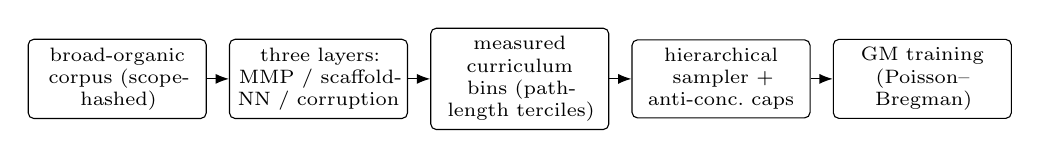
\begin{tikzpicture}[>=Latex, font=\scriptsize, node distance=3pt]
\tikzstyle{b}=[draw, rounded corners=2pt, align=center, inner sep=3pt, minimum height=8mm, text width=2.05cm]
\node[b] (c) {broad-organic corpus (scope-hashed)};
\node[b, right=8pt of c] (l) {three layers: MMP / scaffold-NN / corruption};
\node[b, right=8pt of l] (cur) {measured curriculum bins (path-length terciles)};
\node[b, right=8pt of cur] (s) {hierarchical sampler + anti-conc.\ caps};
\node[b, right=8pt of s] (t) {GM training (Poisson--Bregman)};
\draw[->](c)--(l);\draw[->](l)--(cur);\draw[->](cur)--(s);\draw[->](s)--(t);
\end{tikzpicture}
\caption{Corpus-to-sampler flow. Each stage records a version hash into the data manifest so the corpus
cannot silently drift from the code that produced it.}
\label{fig:dataflow}
\end{figure}

\subsection{Trace layers, compiler, and replay checks}
\emph{Compiled MMP analogue paths.} One-cut matched molecular pairs (constant core; small variable
fragment; bounded atom-count difference; no ring opened across the variable region) are compiled to
executable rewrite programs using mmpdb's constant-fragment and labelled-attachment mapping (not an
unconstrained MCS): preserve the core, delete the source variable fragment leaf-to-root, retype and
reorder as needed, insert the target fragment attachment-outward, replay through the \emph{real} executor,
and check endpoint graph isomorphism, in both directions. \emph{Shared-scaffold analogue paths} connect
each molecule to its $k$ nearest analogue neighbours within a Bemis--Murcko group (sparse nearest
neighbours, never all-pairs cliques). \emph{Corruption paths} walk a real molecule a few reversible legal
edits to a nearby valid source, taught both directions, and are the only layer that exercises the restate,
bond-order, ring, and graft families at pilot scale. Every compiled path is verified for
all-intermediate validity and connectedness, exact endpoint isomorphism, forward and inverse replay,
repeated- and immediately-reversed-edit rates, protected-core invariance, operator-family usage, and the
round-trip $A\!\to\!B\!\to\!A$; a path that reaches the right canonical SMILES but breaks the attachment
mapping or needs gratuitous cycles is rejected. The locked production pool compiles \ConfigValue{PROD_RECORDS}
directed edit records from \ConfigValue{PROD_MMP_PAIRS} one-cut constant-core groups
(\ConfigValue{PROD_RECORDS_FWD} forward / \ConfigValue{PROD_RECORDS_REV} reverse; the compiled pool is exactly
direction-balanced and the residual imbalance is entirely the per-source cap, which keys on each record's
source molecule), with curriculum terciles at path lengths \ConfigValue{CURRICULUM_BIN_EDGES} and the pool,
operator-registry (\ConfigValue{OPERATOR_REGISTRY_HASH}), ring-catalog (\ConfigValue{RING_CATALOG_HASH}), and
standardization (\ConfigValue{STANDARDIZATION_HASH}) hashes pinned in the manifest.

\subsection{Anti-concentration safeguards and curriculum}
Each safeguard has a measured signal and a gate: identity traces are dropped ($\text{identity fraction}
\approx0$); a per-scaffold cap bounds Bemis--Murcko-scaffold Gini and top-$k$ share; a per-transformation
cap and de-duplication bound transformation top-$k$ share; and every enabled family is floored to a
minimum supervised-trace count (rare families are covered by oversampling corruption instances that
exercise them). Curriculum bins are the \emph{measured} terciles of compiled path length
(\ConfigValue{CURRICULUM_BINS}), refined by ring complexity and attachment count---never preset. The
hierarchical sampler draws a layer by its (proposed) mixture weight, then a curriculum bin, then a
balanced example under the caps.

\subsection{Pilot characterization (wiring fixture, not the production mixture)}
At pilot scale (\ConfigValue{PILOT_CORRUPTION_TRACES} corruption traces from real$\to$corrupt and
corrupt$\to$real, and \ConfigValue{PILOT_ANALOGUE_TRACES} analogue traces from
\ConfigValue{PILOT_ANALOGUE_PAIRS} one-cut MMP pairs): the corruption layer has
\ConfigValue{PILOT_CORRUPTION_ACTIVE_FAMILIES} active families, scaffold Gini
\ConfigValue{PILOT_CORRUPTION_SCAFFOLD_GINI}, aromatic-ring change on
\ConfigValue{PILOT_CORRUPTION_AROMATIC_CHANGE_FRAC} of traces, source--target median Tanimoto
\ConfigValue{PILOT_CORRUPTION_TANIMOTO_MEDIAN}, and identity fraction
\ConfigValue{PILOT_CORRUPTION_IDENTITY_FRAC}; the one-cut analogue layer contributes only insert/delete by
construction, which is why a corruption-only or analogue-only corpus is wrong. This pilot pool is a wiring
fixture---its scaffold concentration is too high and its analogue count too small to be the production
analogue layer---and its percentages are \emph{not} the production mixture; the proposed starting shares
(\ConfigValue{MIX_SHARE_CORRUPTION}/\ConfigValue{MIX_SHARE_MMP}/\ConfigValue{MIX_SHARE_SCAFFOLD_NN}) are an
ablation target finalized only from the at-scale statistics. A versioned data manifest records the
partition, standardization and operator-registry hashes, compiler versions, split identifiers, trace
counts, and curriculum-bin definitions.

\subsection{Training}
The edit prior is warm-started from the de novo carbon-tree base checkpoint: shape-compatible body and
embedding parameters transfer, and the wider organic $(\text{element},\text{valence})$ heads (width
\ConfigValue{ORGANIC_VOCAB_SIZE}, versus \ConfigValue{CNOF_VOCAB_SIZE} for the four-element base) retain
the first four transferred rows and freshly initialize the rest, so a four-element checkpoint loads without
a width crash and a de novo checkpoint reloads byte-identically. We state the warm-start honestly: it carries the de novo
ring-growth vocabulary (which the edit layers do not teach) and is a starting point, not the trained edit
prior. Save/reload is exact---a reloaded checkpoint reproduces the sampled mark, hazard, and a fixed-seed
trajectory, and a checkpoint missing required metadata fails loudly. The optimizer, schedule, batch size,
loss normalization, precision, hardware, step budget, checkpoint selection (held-out validation only, never
the test set), and seeds are recorded with each run and released with the code. ``Universal'' means one
edit prior shared across sources and objectives within the declared vocabulary---not all of chemical
space.

\section{Implementation validation}
\label{app:impl}

This appendix reports \emph{implementation-validation} evidence: checks that the code implements the stated
mathematics. These are not headline empirical results (which are the RQ studies of \Cref{sec:experiments},
carried as registry placeholders), and we are careful not to present a passing test as a scientific
finding.

\subsection{Enumerable-benchmark construction and Doob residuals}
The enumerable chain is built by breadth-first expansion of the real legal fiber from methane, capping
successors at \ConfigValue{E0_ENUM_MAX_HEAVY} heavy atoms, yielding a \ConfigValue{E0_ENUM_STATES}-state
row-stochastic embedded kernel over canonical molecular states. On this chain the finite-horizon Doob
transform is verified against its closed form: the controlled terminal law matches the analytic tilt to
total variation \ConfigValue{DOOB_ENUM_TV_RESIDUAL} (\Cref{thm:doob}); dynamic-retargeting continuation
matches the $\desir'$-tilt from the switch state to \ConfigValue{DYNAMIC_ENUM_TV_RESIDUAL}
(\Cref{cor:dynamic}); and an early-stop marginal is confirmed \emph{not} to equal the terminal tilt
(TV~$>2\times10^{-2}$ two steps early), so exactness is budget-specific. No sampled controlled transition
leaves the base support.

\subsection{Kernel, measure, and quotient}
The successor-sampling kernel of the canonical-successor quotient sampler equals the raw mark sampler's
induced kernel to $<\ConfigValue{QUOTIENT_KERNEL_EQ_TOL}$ on tree, symmetric-tree, self-graft, cyclic, and
post-ring-opening states (\Cref{prop:kernel}); the mark law is a proper distribution ($\sum_a\pmark(a\mid
x)=1$ to $\sim10^{-7}$ on every molecule tested), Graft group mass equals the sum of its successor-group
rates, and Monte-Carlo successor frequencies agree within the null band with no out-of-support draws.

\subsection{Objective, gradients, and tiny-corpus convergence}
On a tiny verified corpus over distinct states (no conflicting targets), the Poisson--Bregman loss
descends from \ConfigValue{TINY_OVERFIT_LOSS_INITIAL} to \ConfigValue{TINY_OVERFIT_LOSS_FINAL}, within
$0.14$ of the per-example lower bound \ConfigValue{TINY_OVERFIT_LOWER_BOUND}, and every production family's
selected-mark probability rises---so each enabled head receives a finite, non-suppressive gradient from a
positive teacher, and the model can overfit the verified corpus. This is a wiring check, not a quality
claim.

\subsection{Closure, charge, save/reload, held-out rollouts}
A random legal-edit fuzz produces valid, connected successors across families (\Cref{prop:closure});
charged, drug-like leads round-trip with net charge and charged centers preserved (no edit changes a
formal charge); save/reload is exact and reconstructs the organic vocabulary and editing capabilities from
checkpoint metadata (a de novo checkpoint reloads byte-identically; a checkpoint missing required metadata
fails loudly); and over held-out drug-like leads at budgets $1$--$8$, rollouts start at the lead (never a
carbon-tree seed), recompute the legal set per state, commit only executor-accepted edits, and maintain
$100\%$ all-intermediate validity and connectivity. The degeneracy/reversal diagnostics are measured for
plumbing; their \emph{quality} reading requires the trained model.

\subsection{Test suite and clean-lineage provenance}
The committed suite passes on a pristine worktree (recorded gates: \ConfigValue{GATE_TESTS_AUDIT} at the
audited commit and \ConfigValue{GATE_TESTS_STAGE6} at the Stage-6 commit; the count grows with each added
check). The evidence lineage for this manuscript is commit \ConfigValue{EVIDENCE_COMMIT} on the clean
lineage tagged \ConfigValue{EVIDENCE_TAG}. Pre-fix editing outputs (which sampled the de novo vocabulary
for an edit checkpoint) are treated as stale and are never cited.

\subsection{Legacy-sampler correctness diagnostic (not a competitor)}
A prior sampler variant normalized the Graft family over the raw (self-graft-inclusive) partition rather
than the quotient partition, giving a graft family rate that disagreed with training (e.g.\ $0.097$ vs
$0.136$ on octane). This is retained only as a named historical ablation to \emph{diagnose} the quotient
convention; it is not a controller and is never run as a baseline in \Cref{sec:experiments}, because a
known-incorrect sampler is not a fair scientific competitor.

\section{Extended experimental protocol}
\label{app:experiments}

This appendix gives the full protocol behind \Cref{sec:experiments}: metric definitions stated before any
result, per-baseline documentation, and the figure/table scaffolds. All empirical cells are result-registry
placeholders.

\subsection{RQ1 panels (enumerable benchmark)}
Each conditioning task is evaluated by total variation between a method's controlled terminal law and the
exact target: exact Doob (\Result{E0_EXACT_TV}, with maximum per-state error \Result{E0_EXACT_MAX_ERROR}),
the learned controller (\Result{E0_LEARNED_TV}), one-step greedy (\Result{E0_GREEDY_TV}), endpoint
reranking (\Result{E0_RERANK_TV}), and dynamic retargeting (\Result{E0_DYNAMIC_TV}); the target-event-%
probability error under indicator conditioning is \Result{E0_EVENT_ERROR}, and support violations are
\Result{E0_SUPPORT_VIOLATIONS} (zero by construction).

\begin{figure}[h]
\centering
\pendingfigure{3.0cm}{Panels: (a) unconditioned vs desired-tilted vs exact-Doob vs greedy endpoint
histograms on the enumerable chain; (b) TV to the exact law per method; (c) $\hval_\phi$ calibration vs
exact $\hval$; (d) backward-equation residual vs training. Rendered from the enumerable-benchmark artifact.}
\caption{\textbf{Exactness on the enumerable chemical state space (RQ1).} Exact Doob is expected to match
the analytic target to numerical precision while reward-local controllers attain high reward at a
different distribution; the figure is populated from the enumerable-benchmark artifact when the run
completes.}
\label{fig:e0}
\end{figure}

\subsection{Adaptation regret (defined before results)}
For a preference switch to $\descr'$ at trajectory fraction $\tau/\horizon$, let $U_{\descr'}$ be the new
utility and $U^\star_{\descr'}(x_\tau,b)$ the best achievable expected utility from state $x_\tau$ with
remaining budget $b=\horizon-\tau$ under the base process. The \emph{adaptation regret} of a method that
reaches terminal utility $U_{\descr'}(X_\horizon)$ is $R=U^\star_{\descr'}(x_\tau,b)-\Ebb[U_{\descr'}
(X_\horizon)]$, estimated with the exact controller as the reference on enumerable slices and with a
matched-budget oracle-best on real leads; lower is better. Steps-to-region counts committed edits until
$\Fobj(X_k)\in\Bset_{\descr'}$, and retention is the fraction of the pre-switch objective's gain preserved
at the terminal state. These are fixed here so RQ3 reports them without post-hoc definition.

\subsection{Per-baseline documentation}
\emph{Same-base controllers} (all steer the identical canonical-successor kernel $\Ptheta$): \emph{unguided}
samples $\Ptheta$; \emph{endpoint$+$rerank} samples $\Ptheta$ and reranks terminal candidates by the
objective; \emph{greedy $\Delta\Fobj$} picks the successor of maximal immediate objective gain;
\emph{local Boltzmann} reweights $\Ptheta$ by $\exp(\beta\Delta\Fobj)$; \emph{MOG-DFM-style} applies a
rank-directional score with an adaptive hypercone filter over $\Ptheta$'s successors; \emph{SMC/Feynman--Kac}
runs a twisted-SMC population with resampling; \emph{learned Doob} uses \eqref{eq:controlledphi}. \emph{External
optimizers} (contextual; Table~\ref{tab:h1ext}): GraphGA (graph genetic algorithm), MARS (annealed
fragment-edit MCMC), GenMol (masked discrete-diffusion generalist), and RetMol (retrieval-controlled
generation); each is run at a matched oracle budget with its released configuration, and where possible
additionally over our legal proposal set to separate the control law from the edit vocabulary. Any
asymmetric tuning is disclosed with the result.

\subsection{Hypervolume hygiene}
Objective bounds and the reference point are fixed before evaluation and published; the archive is capped
per method; hypervolume is reported against oracle calls (HV-AUC), not only at the final budget; and
hypervolume is paired with IGD+ and coverage so a single indicator does not carry the claim. All oracle
evaluations---including intermediates, rejected, invalid, reranked, and SMC particles---are counted
(\Cref{sec:fairness}).

\subsection{Secondary: de novo generation}
De novo generation from the target-independent carbon-tree prior is evaluated on all-step validity
(\Result{DENOVO_VALIDITY}), uniqueness, novelty, Fr\'echet ChemNet Distance (\Result{DENOVO_FCD}), and
property divergence, as evidence that the operators form a genuine generative process. It is secondary; the
paper's claims do not depend on carbon-tree intermediates being useful lead-optimization states.

% H1 external optimizers (appendix). Contextual comparison; differ in scale and
% representation. Every cell is a result-registry placeholder.
\begin{table}[h]
\centering
\caption{\textbf{RQ2 external optimizers (contextual).} These methods differ from ours in scale and
representation, so they contextualize rather than isolate the control law; where possible each is
additionally run on our legal proposal set (\Cref{sec:fairness}). Same conventions and reference point as
Table~\ref{tab:h1}; the Diversity column (internal diversity of the nondominated set) is included here
for completeness. Placeholders are filled from the registry when the runs complete.}
\label{tab:h1ext}
\footnotesize
\setlength{\tabcolsep}{3.6pt}
\begin{tabular}{l ccccccc}
\toprule
Method & nHV\,$\uparrow$ & HV-AUC\,$\uparrow$ & IGD+\,$\downarrow$ & \#Feas\,$\uparrow$
       & Src-sim\,$\uparrow$ & Div\,$\uparrow$ & Orc-eff\,$\uparrow$ \\
\midrule
GraphGA & \Result{H1_NHV_GRAPHGA} & \Result{H1_HVAUC_GRAPHGA} & \Result{H1_IGD_GRAPHGA} & \Result{H1_FEASIBLE_GRAPHGA} & \Result{H1_SOURCESIM_GRAPHGA} & \Result{H1_DIVERSITY_GRAPHGA} & \Result{H1_ORACLEEFF_GRAPHGA}\\
MARS & \Result{H1_NHV_MARS} & \Result{H1_HVAUC_MARS} & \Result{H1_IGD_MARS} & \Result{H1_FEASIBLE_MARS} & \Result{H1_SOURCESIM_MARS} & \Result{H1_DIVERSITY_MARS} & \Result{H1_ORACLEEFF_MARS}\\
GenMol & \Result{H1_NHV_GENMOL} & \Result{H1_HVAUC_GENMOL} & \Result{H1_IGD_GENMOL} & \Result{H1_FEASIBLE_GENMOL} & \Result{H1_SOURCESIM_GENMOL} & \Result{H1_DIVERSITY_GENMOL} & \Result{H1_ORACLEEFF_GENMOL}\\
RetMol & \Result{H1_NHV_RETMOL} & \Result{H1_HVAUC_RETMOL} & \Result{H1_IGD_RETMOL} & \Result{H1_FEASIBLE_RETMOL} & \Result{H1_SOURCESIM_RETMOL} & \Result{H1_DIVERSITY_RETMOL} & \Result{H1_ORACLEEFF_RETMOL}\\
\multicolumn{8}{l}{\emph{Same-base controllers (Table~\ref{tab:h1}) additionally with the Diversity column:}}\\
Learned Doob (ours) & \Result{H1_NHV_LEARNEDDOOB} & \Result{H1_HVAUC_LEARNEDDOOB} & \Result{H1_IGD_LEARNEDDOOB} & \Result{H1_FEASIBLE_LEARNEDDOOB} & \Result{H1_SOURCESIM_LEARNEDDOOB} & \Result{H1_DIVERSITY_LEARNEDDOOB} & \Result{H1_ORACLEEFF_LEARNEDDOOB}\\
\bottomrule
\end{tabular}
\end{table}

% Pareto fan (RQ3). Renders from a real dynamic-steering run: every displayed
% molecule is from an actual trajectory; any selection among branches is disclosed.
\begin{figure}[t]
\centering
\pendingfigure{2.5cm}{One lead $\xsrc$; a shared controlled prefix; then a fan of
preference-conditioned valid branches (one per goal $\descr$), each ending in a committed molecule.
Molecules rendered from a real run; branch selection, if any, disclosed here.}
\caption{\textbf{Dynamic preference steering: the Pareto fan (RQ3).} From a single source lead, a shared
controlled prefix fans into several preference-conditioned trajectories via exact continuation
(\Cref{cor:dynamic}); each branch is a distinct goal descriptor $\descr$ applied to the remaining budget,
and every committed state along every branch is a complete, valid molecule. The panel is populated from
one real dynamic-steering run over a single lead across $8$--$16$ preferences; molecules shown are actual
trajectory states (no cherry-picked composites), and any down-selection among branches for legibility is
stated in this caption when the figure is rendered. No numerical results are asserted here until the run
completes.}
\label{fig:fan}
\end{figure}


\section{Large language model use}
\label{app:llm}

We disclose the use of large language models (LLMs) in preparing this work, factually and specifically. An
LLM is not an author and made no scientific decisions. LLM assistance was used for: (i) drafting and
copy-editing prose from author-provided technical content, notation, and results, which the authors then
verified line by line against the implementation and the mathematics; (ii) assisting a literature search
whose every citation was subsequently verified by the authors against a primary source (arXiv, OpenReview,
or a publisher DOI), with venue and author details corrected where the model erred; and (iii) routine code
and tooling assistance (for example, the result-placeholder build system) under author review and the
project's test suite. All theorem statements, proofs, experimental designs, claims, and their evidentiary
status were determined and checked by the authors; the LLM did not generate any empirical number, and the
result-registry system exists precisely so that no value enters the manuscript without a machine-readable
artifact behind it. The authors take full responsibility for the entire content, including any remaining
errors.

\section{Anonymous-release checklist}
\label{app:repromap}

A code and data release accompanying this paper will be scrubbed for double-blind review against the
following checklist before posting; each item is a required pre-release check. \emph{Identity:} remove
author and affiliation names, acknowledgements, and grant numbers; remove any user, account, or cluster
names. \emph{Paths and infrastructure:} rewrite absolute home-directory paths, remove cloud-profile and
compute-account names, and strip internal hostnames and repository remotes. \emph{Self-citation:} phrase
all references to prior work by the same authors in the third person and remove links that would reveal
identity through a personal or lab domain. \emph{Artifacts:} scrub PDF metadata (author, title, producer),
strip identifying strings from supplementary archives and notebooks, and remove identifying comments and
environment files from the code. \emph{Links:} replace tracking or identity-revealing URLs with anonymized
mirrors. \emph{Terminology:} the manuscript uses only public method terminology (base prior, edit prior,
canonical successor kernel, controlled editing process, source-conditioned controller); internal
engineering codenames are confined to the authors' private reproducibility notes and never appear in the
released paper or code comments. The released bundle will include the result registry, the plotting
artifacts backing every figure and table, the enumerable-benchmark harness, and the data manifest with its
scope and operator-registry hashes, so that every claim in the paper maps to a runnable check.


\end{document}
